% !TeX encoding = UTF-8
% *** Authors should verify (and, if needed, correct) their LaTeX system  ***
% *** with the testflow diagnostic prior to trusting their LaTeX platform ***
% *** with production work. IEEE's font choices and paper sizes can       ***
% *** trigger bugs that do not appear when using other class files.       ***                          ***
% The testflow support page is at:
% http://www.michaelshell.org/tex/testflow/

\documentclass[journal,twoside]{IEEEtran}

% Some very useful LaTeX packages include:
% (uncomment the ones you want to load)

% *** CITATION PACKAGES ***
%
\usepackage{cite}
% cite.sty was written by Donald Arseneau
% V1.6 and later of IEEEtran pre-defines the format of the cite.sty package
% \cite{} output to follow that of IEEE. Loading the cite package will
% result in citation numbers being automatically sorted and properly
% "compressed/ranged". e.g., [1], [9], [2], [7], [5], [6] without using
% cite.sty will become [1], [2], [5]--[7], [9] using cite.sty. cite.sty's
% \cite will automatically add leading space, if needed. Use cite.sty's
% noadjust option (cite.sty V3.8 and later) if you want to turn this off
% such as if a citation ever needs to be enclosed in parenthesis.
% cite.sty is already installed on most LaTeX systems. Be sure and use
% version 5.0 (2009-03-20) and later if using hyperref.sty.
% The latest version can be obtained at:
% http://www.ctan.org/tex-archive/macros/latex/contrib/cite/
% The documentation is contained in the cite.sty file itself.

% *** GRAPHICS RELATED PACKAGES ***
%
\ifCLASSINFOpdf
   \usepackage[pdftex]{graphicx}
  % declare the path(s) where your graphic files are
   \graphicspath{{./images/}}
  % and their extensions so you won't have to specify these with
  % every instance of \includegraphics
   \DeclareGraphicsExtensions{.pdf,.jpeg,.png}
\else
  % or other class option (dvipsone, dvipdf, if not using dvips). graphicx
  % will default to the driver specified in the system graphics.cfg if no
  % driver is specified.
  % \usepackage[dvips]{graphicx}
  % declare the path(s) where your graphic files are
  % \graphicspath{{../eps/}}
  % and their extensions so you won't have to specify these with
  % every instance of \includegraphics
  % \DeclareGraphicsExtensions{.eps}
\fi
% graphicx was written by David Carlisle and Sebastian Rahtz. It is
% required if you want graphics, photos, etc. graphicx.sty is already
% installed on most LaTeX systems. The latest version and documentation
% can be obtained at: 
% http://www.ctan.org/tex-archive/macros/latex/required/graphics/
% Another good source of documentation is "Using Imported Graphics in
% LaTeX2e" by Keith Reckdahl which can be found at:
% http://www.ctan.org/tex-archive/info/epslatex/
%
% latex, and pdflatex in dvi mode, support graphics in encapsulated
% postscript (.eps) format. pdflatex in pdf mode supports graphics
% in .pdf, .jpeg, .png and .mps (metapost) formats. Users should ensure
% that all non-photo figures use a vector format (.eps, .pdf, .mps) and
% not a bitmapped formats (.jpeg, .png). IEEE frowns on bitmapped formats
% which can result in "jaggedy"/blurry rendering of lines and letters as
% well as large increases in file sizes.
%
% You can find documentation about the pdfTeX application at:
% http://www.tug.org/applications/pdftex

% *** MATH PACKAGES ***
%
\usepackage[cmex10]{amsmath}
% A popular package from the American Mathematical Society that provides
% many useful and powerful commands for dealing with mathematics. If using
% it, be sure to load this package with the cmex10 option to ensure that
% only type 1 fonts will utilized at all point sizes. Without this option,
% it is possible that some math symbols, particularly those within
% footnotes, will be rendered in bitmap form which will result in a
% document that can not be IEEE Xplore compliant!
%
% Also, note that the amsmath package sets \interdisplaylinepenalty to 10000
% thus preventing page breaks from occurring within multiline equations. Use:
%\interdisplaylinepenalty=2500
% after loading amsmath to restore such page breaks as IEEEtran.cls normally
% does. amsmath.sty is already installed on most LaTeX systems. The latest
% version and documentation can be obtained at:
% http://www.ctan.org/tex-archive/macros/latex/required/amslatex/math/

% *** SPECIALIZED LIST PACKAGES ***
%
%\usepackage{algorithmic}
% algorithmic.sty was written by Peter Williams and Rogerio Brito.
% This package provides an algorithmic environment fo describing algorithms.
% You can use the algorithmic environment in-text or within a figure
% environment to provide for a floating algorithm. Do NOT use the algorithm
% floating environment provided by algorithm.sty (by the same authors) or
% algorithm2e.sty (by Christophe Fiorio) as IEEE does not use dedicated
% algorithm float types and packages that provide these will not provide
% correct IEEE style captions. The latest version and documentation of
% algorithmic.sty can be obtained at:
% http://www.ctan.org/tex-archive/macros/latex/contrib/algorithms/
% There is also a support site at:
% http://algorithms.berlios.de/index.html
% Also of interest may be the (relatively newer and more customizable)
% algorithmicx.sty package by Szasz Janos:
% http://www.ctan.org/tex-archive/macros/latex/contrib/algorithmicx/

% *** ALIGNMENT PACKAGES ***
%
\usepackage{array}
% Frank Mittelbach's and David Carlisle's array.sty patches and improves
% the standard LaTeX2e array and tabular environments to provide better
% appearance and additional user controls. As the default LaTeX2e table
% generation code is lacking to the point of almost being broken with
% respect to the quality of the end results, all users are strongly
% advised to use an enhanced (at the very least that provided by array.sty)
% set of table tools. array.sty is already installed on most systems. The
% latest version and documentation can be obtained at:
% http://www.ctan.org/tex-archive/macros/latex/required/tools/


% IEEEtran contains the IEEEeqnarray family of commands that can be used to
% generate multiline equations as well as matrices, tables, etc., of high
% quality.

% *** SUBFIGURE PACKAGES ***
%\ifCLASSOPTIONcompsoc
%  \usepackage[caption=false,font=normalsize,labelfont=sf,textfont=sf]{subfig}
%\else
%  \usepackage[caption=false,font=footnotesize]{subfig}
%\fi
% subfig.sty, written by Steven Douglas Cochran, is the modern replacement
% for subfigure.sty, the latter of which is no longer maintained and is
% incompatible with some LaTeX packages including fixltx2e. However,
% subfig.sty requires and automatically loads Axel Sommerfeldt's caption.sty
% which will override IEEEtran.cls' handling of captions and this will result
% in non-IEEE style figure/table captions. To prevent this problem, be sure
% and invoke subfig.sty's "caption=false" package option (available since
% subfig.sty version 1.3, 2005/06/28) as this is will preserve IEEEtran.cls
% handling of captions.
% Note that the Computer Society format requires a larger sans serif font
% than the serif footnote size font used in traditional IEEE formatting
% and thus the need to invoke different subfig.sty package options depending
% on whether compsoc mode has been enabled.
%
% The latest version and documentation of subfig.sty can be obtained at:
% http://www.ctan.org/tex-archive/macros/latex/contrib/subfig/

% *** FLOAT PACKAGES ***
%
%\usepackage{fixltx2e}
% fixltx2e, the successor to the earlier fix2col.sty, was written by
% Frank Mittelbach and David Carlisle. This package corrects a few problems
% in the LaTeX2e kernel, the most notable of which is that in current
% LaTeX2e releases, the ordering of single and double column floats is not
% guaranteed to be preserved. Thus, an unpatched LaTeX2e can allow a
% single column figure to be placed prior to an earlier double column
% figure. The latest version and documentation can be found at:
% http://www.ctan.org/tex-archive/macros/latex/base/

%\usepackage{stfloats}
% stfloats.sty was written by Sigitas Tolusis. This package gives LaTeX2e
% the ability to do double column floats at the bottom of the page as well
% as the top. (e.g., "\begin{figure*}[!b]" is not normally possible in
% LaTeX2e). It also provides a command:
%\fnbelowfloat
% to enable the placement of footnotes below bottom floats (the standard
% LaTeX2e kernel puts them above bottom floats). This is an invasive package
% which rewrites many portions of the LaTeX2e float routines. It may not work
% with other packages that modify the LaTeX2e float routines. The latest
% version and documentation can be obtained at:
% http://www.ctan.org/tex-archive/macros/latex/contrib/sttools/
% Do not use the stfloats baselinefloat ability as IEEE does not allow
% \baselineskip to stretch. Authors submitting work to the IEEE should note
% that IEEE rarely uses double column equations and that authors should try
% to avoid such use. Do not be tempted to use the cuted.sty or midfloat.sty
% packages (also by Sigitas Tolusis) as IEEE does not format its papers in
% such ways.
% Do not attempt to use stfloats with fixltx2e as they are incompatible.
% Instead, use Morten Hogholm'a dblfloatfix which combines the features
% of both fixltx2e and stfloats:
%
% \usepackage{dblfloatfix}
% The latest version can be found at:
% http://www.ctan.org/tex-archive/macros/latex/contrib/dblfloatfix/

%\ifCLASSOPTIONcaptionsoff
%  \usepackage[nomarkers]{endfloat}
% \let\MYoriglatexcaption\caption
% \renewcommand{\caption}[2][\relax]{\MYoriglatexcaption[#2]{#2}}
%\fi
% endfloat.sty was written by James Darrell McCauley, Jeff Goldberg and 
% Axel Sommerfeldt. This package may be useful when used in conjunction with 
% IEEEtran.cls'  captionsoff option. Some IEEE journals/societies require that
% submissions have lists of figures/tables at the end of the paper and that
% figures/tables without any captions are placed on a page by themselves at
% the end of the document. If needed, the draftcls IEEEtran class option or
% \CLASSINPUTbaselinestretch interface can be used to increase the line
% spacing as well. Be sure and use the nomarkers option of endfloat to
% prevent endfloat from "marking" where the figures would have been placed
% in the text. The two hack lines of code above are a slight modification of
% that suggested by in the endfloat docs (section 8.4.1) to ensure that
% the full captions always appear in the list of figures/tables - even if
% the user used the short optional argument of \caption[]{}.
% IEEE papers do not typically make use of \caption[]'s optional argument,
% so this should not be an issue. A similar trick can be used to disable
% captions of packages such as subfig.sty that lack options to turn off
% the subcaptions:
% For subfig.sty:
% \let\MYorigsubfloat\subfloat
% \renewcommand{\subfloat}[2][\relax]{\MYorigsubfloat[]{#2}}
% However, the above trick will not work if both optional arguments of
% the \subfloat command are used. Furthermore, there needs to be a
% description of each subfigure *somewhere* and endfloat does not add
% subfigure captions to its list of figures. Thus, the best approach is to
% avoid the use of subfigure captions (many IEEE journals avoid them anyway)
% and instead reference/explain all the subfigures within the main caption.
% The latest version of endfloat.sty and its documentation can obtained at:
% http://www.ctan.org/tex-archive/macros/latex/contrib/endfloat/
%
% The IEEEtran \ifCLASSOPTIONcaptionsoff conditional can also be used
% later in the document, say, to conditionally put the References on a 
% page by themselves.

% *** PDF, URL AND HYPERLINK PACKAGES ***
%
\usepackage{url}
% url.sty was written by Donald Arseneau. It provides better support for
% handling and breaking URLs. url.sty is already installed on most LaTeX
% systems. The latest version and documentation can be obtained at:
% http://www.ctan.org/tex-archive/macros/latex/contrib/url/
% Basically, \url{my_url_here}.

% *** Do not adjust lengths that control margins, column widths, etc. ***
% *** Do not use packages that alter fonts (such as pslatex).         ***
% There should be no need to do such things with IEEEtran.cls V1.6 and later.
% (Unless specifically asked to do so by the journal or conference you plan
% to submit to, of course. )

% correct bad hyphenation here
\hyphenation{op-tical net-works semi-conduc-tor}

% ***ADDED BY JONAS***
\usepackage{wrapfig}
\usepackage{url}
\usepackage{nohyperref}
%for columns spanning multiple rows in tables
\usepackage{multirow}
%use the booktabs package to get (much!) better vertical spacing above and below "rules" (horizontal lines), resulting in a much more professional look of your tables.
%use the colortbl package to add color to tables.
\usepackage{booktabs,colortbl}

\usepackage{amsfonts}

\renewcommand{\vec}[1]{\mathbf{#1}}
% ********************

\begin{document}
%
% paper title
% Titles are generally capitalized except for words such as a, an, and, as,
% at, but, by, for, in, nor, of, on, or, the, to and up, which are usually
% not capitalized unless they are the first or last word of the title.
% Linebreaks \\ can be used within to get better formatting as desired.
% Do not put math or special symbols in the title.
\title{Temporal Instanton Analysis:\\
Development and Implementation}
%
%
% author names and IEEE memberships
% note positions of commas and nonbreaking spaces ( ~ ) LaTeX will not break
% a structure at a ~ so this keeps an author's name from being broken across
% two lines.
% use \thanks{} to gain access to the first footnote area
% a separate \thanks must be used for each paragraph as LaTeX2e's \thanks
% was not built to handle multiple paragraphs
%

\author{Jonas~A.~Kersulis,~\IEEEmembership{Student~Member,~IEEE,}
        and~Ian~A.~Hiskens,~\IEEEmembership{Fellow,~IEEE}% <-this % stops a space
\thanks{The authors are with the Department of Electrical Engineering and Computer Science, University of Michigan, Ann Arbor, MI 48104 USA (e-mail: 
kersulis@umich.edu; hiskens@umich.edu)}%
\thanks{This work was supported by the Los Alamos National Laboratory Grid Science Program, subcontract 270958.}}
%\thanks{Manuscript received ____; revised __.}}

% note the % following the last \IEEEmembership and also \thanks - 
% these prevent an unwanted space from occurring between the last author name
% and the end of the author line. i.e., if you had this:
% 
% \author{....lastname \thanks{...} \thanks{...} }
%                     ^------------^------------^----Do not want these spaces!
%
% a space would be appended to the last name and could cause every name on that
% line to be shifted left slightly. This is one of those "LaTeX things". For
% instance, "\textbf{A} \textbf{B}" will typeset as "A B" not "AB". To get
% "AB" then you have to do: "\textbf{A}\textbf{B}"
% \thanks is no different in this regard, so shield the last } of each \thanks
% that ends a line with a % and do not let a space in before the next \thanks.
% Spaces after \IEEEmembership other than the last one are OK (and needed) as
% you are supposed to have spaces between the names. For what it is worth,
% this is a minor point as most people would not even notice if the said evil
% space somehow managed to creep in.

% The paper headers
\markboth{IEEE Transactions on Power Systems,~Vol.~--, No.~-, ---~201-}%
{Kersulis and Hiskens: Temporal Instanton Analysis}
% The only time the second header will appear is for the odd numbered pages
% after the title page when using the twoside option.
% 
% *** Note that you probably will NOT want to include the author's ***
% *** name in the headers of peer review papers.                   ***
% You can use \ifCLASSOPTIONpeerreview for conditional compilation here if
% you desire.

% make the title area
\maketitle

% As a general rule, do not put math, special symbols or citations
% in the abstract or keywords.
\begin{abstract}
%A time-coupled instanton method for characterizing transmission network vulnerability to wind generation fluctuation is presented. To extend prior instanton work to multiple-time-step analysis, line constraints are specified in terms of temperature rather than current. An optimization formulation is developed to express the minimum wind forecast deviation such that at least one line is driven to its thermal limit. Results are shown for an IEEE RTS-96 system with several wind-farms.
A previously-developed method for studying a transmission network's vulnerability to wind forecast inaccuracy is expanded. The method uses optimization to find a likely wind generation pattern that brings a specified line to an unacceptably high temperature. The objective quantifies wind pattern likelihood in terms of distance from the forecast, respecting spatial and temporal correlation between wind sites and time intervals. The set of constraints enforces power balance and ensures a chosen line in the network reaches a fixed temperature by the final time step. The thermal constraint is second-order in voltage angle differences, and is based on a DC-approximate line loss formulation. Repeatedly solving the QCQP for all lines in the network yields a set of instanton candidate generation patterns, which may then be sorted by likelihood. Having described the temporal instanton QCQP and its solution, the paper turns to a discussion of implementation details. Finally, a series of numerical experiments is presented. These experiments demonstrate the effect of an instanton pattern on line temperature trajectory, the effects of wind covariance on instanton analysis, and algorithm scaling properties.
\end{abstract}

% Note that keywords are not normally used for peerreview papers.
\begin{IEEEkeywords}
forecast uncertainty, optimization, transmission operations, wind energy
\end{IEEEkeywords}

% For peer review papers, you can put extra information on the cover
% page as needed:
% \ifCLASSOPTIONpeerreview
% \begin{center} \bfseries EDICS Category: 3-BBND \end{center}
% \fi
%
% For peerreview papers, this IEEEtran command inserts a page break and
% creates the second title. It will be ignored for other modes.
\IEEEpeerreviewmaketitle

\section{Introduction}\label{sec:intro}
\IEEEPARstart{A}{wind} forecast error that was once inconsequential is now vexatious. As wind grows into a major transmission-scale energy source, system operators find themselves frequently dealing with wind-induced network congestion \cite{rogers2010}. Operators use wind forecast data to steer the network, but wind forecasts are significantly less accurate than generation and demand predictions \cite{parsons2004}. Might forecast deviations compound across a collection of wind farms to overheat a transmission line? Which lines are most vulnerable to such an event? Temporal instanton analysis addresses these questions by identifying sag-inducing wind patterns and ranking them according to likelihood. The intersection of likely wind patterns with those that cause excessive line heating is of interest to system operators and planners, who may use this information to better prepare for renewable generation uncertainty.

Instanton analysis belongs to the family of distance to failure algorithms. It was introduced in \cite{chertkov2011} and \cite{chertkov2011a}, where the DC power flow approximation was used to represent a network's feasible operating region as a set of linear constraints. These constraints form the faces of a high-dimensional polytope that contains all feasible network states. Distance to failure is intuitively understood to be the shortest distance between an operating point and the surface of the constraint polytope. As shown in \cite{chertkov2011a}, one can use convex optimization to quickly find the smallest shift in wind generation that will drive the network to a chosen polytope face. Once every face has been considered, the collection of shifts may be sorted by distance from the forecast operating point. The wind pattern corresponding to the shortest distance between the forecast operating point and the boundary of the constraint polytope is termed the instanton; it is the smallest shift in wind generation that will drive the network to the brink of infeasibility.

%\begin{wrapfigure}{r}{0.45\linewidth}
%\centering
%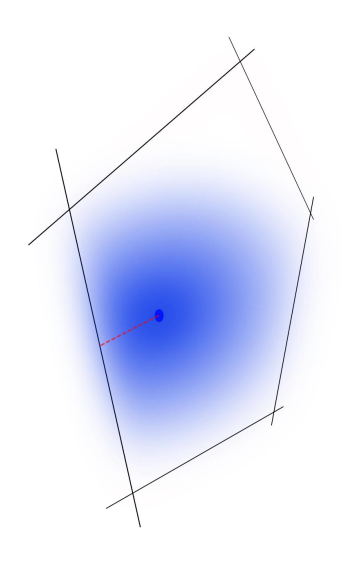
\includegraphics[width=0.5\linewidth]{../images/stylizedFeas}
%\caption{}
%\label{fig:stylizedFeas}
%\end{wrapfigure}
\begin{figure}
\centering
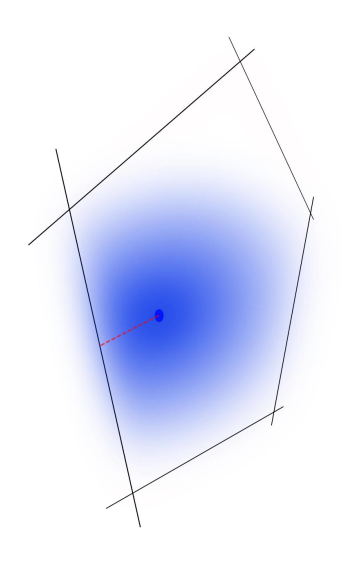
\includegraphics[angle=90,width=0.64\linewidth]{../images/stylizedFeas}
\caption{How far is the forecast operating point from the edge of the feasible region, and might forecast inaccuracies drive the system there?}
\label{fig:stylizedFeas}
\end{figure}


Instanton analysis research falls into two categories. The first is exploration of the trade-off between accuracy and algorithm complexity. Replacing the DC power flow approximation with the full AC model, for instance, yields greater accuracy at the cost of convexity \cite{baghsorkhi2012}. Between the DC and AC extremes are various power flow approximations (see \cite{coffrin2012,hijazi2013,coffrin2014} for examples) which may be used to enhance accuracy while maintaining the solution guarantees of convexity. Regardless of the power flow model used, research in this category is ultimately focused on instantaneous vulnerability: find the smallest wind generation shift that drives a line to its steady-state power or current limit. This method uncovers previously hidden grid vulnerability, but it is safe to briefly operate a line above its current limit. As long as the line is allowed to cool before sagging to some limit (defined by statute and nearby trees), no harm is done. System operators know this; they periodically allow lines to operate above their rated steady-state limits to promote smooth operation during congestion \cite{banakar2005}. Thus, if an operator is comfortable with temporarily overloaded lines, information from instantaneous instanton analysis may be too conservative to aid decision making. Temporal instanton analysis, the second research category, seeks to overcome this limitation by accommodating multiple time steps.


In this paper we expound on the temporal instanton analysis method introduced in \cite{kersulis2015}. By modeling line temperature over an appropriate time horizon, the proposed method discovers multiple-time-step wind patterns that are both likely to occur and sure to bring at least one line in the network to its temperature limit. The remainder of this paper is organized as follows. Section \ref{sec:models} describes the models at the core of temporal instanton analysis. Section \ref{sec:qcqp} combines these models into a quadratically-constrained quadratic program (QCQP). The solution of this QCQP is described in Section \ref{sec:solution}. Section \ref{sec:implementation}  contains results for two networks: a modified version of the RTS-96 and the larger WECC network. The former network has been used in previous instanton analysis studies, while the latter serves to demonstrate scalability of temporal instanton analysis. Finally, an appendix contains a detailed description of the thermal model used to calculate line temperature.

We expand on prior work by providing a more detailed treatment of the objective function, discussing implementation details including computational complexity and sparsity, and proposing a particular algorithm for solving the secular equation.

\section{Models}\label{sec:models}
Temporal instanton analysis entwines three physical phenomena, each requiring a model. Transmission line temperature is based on a heat balance model, forecast error likelihood is quantified via a statistical model, and the feasible region of network operation is delineated using a network model. This section describes the three models in detail. The next section combines them into a quadratically-constrained quadratic program. Temporal instanton analysis consists of solving this QCQP for each line in a network.

% a brief note on notation

\subsection{Transmission Line Heating}\label{sec:models-heat}
A simplified relationship between power flow and line temperature is key to making temporal instanton analysis tractable. Starting with an IEEE standard \cite{ieee2013}, we derive an approximate recursive relationship between a line's temperature at one time step and voltage angle differences at all previous time steps. This relation is summarized below (and the Appendix contains a detailed derivation).

Consider a time horizon with $n$ intervals, each on the order of ten minutes long. Power flow data is updated once per interval, but all other parameters (resistance, solar heating, etc.) remain constant. Choose a single transmission line in the network ---suppose it lies between nodes $i$ and $j$--- and let this line's thermal limit be represented by $T_\text{lim,C}$ ($^\circ$C). We can constrain the line's temperature at the end of the $T$-th interval to be equal to this limiting value by enforcing the second-order constraint
\begin{align}\label{eq:tempconstraint}
\sum_{k=1}^n \hat{\theta}_{ij}(t_k)^2 &= \frac{a}{c}\left(T_\text{lim,C} - f\right),
\end{align}
where
\begin{subequations}\label{eq:heatbreakdown}
\begin{align}
\label{eq:heatbreakdown-theta}\hat{\theta}_{ij}(t_{k}) &= \theta_{ij}(t_k)\sqrt{ (e^{a\bar{t}})^{n-k+1} - (e^{a\bar{t}})^{n-k} } \\
\label{eq:heatbreakdown-a}a &= \frac{1}{mC_p}\left[ -\eta_c - 4\eta_r T_\text{m,K}^3 \right] \\
\label{eq:heatbreakdown-c}c &= \frac{r_{ij}S_b}{3 mC_p x_{ij}^2L_{ij}} \\
\label{eq:heatbreakdown-d}d &= \frac{ \eta_cT_\text{a,C} + \eta_r\big( 4T_\text{m,C}T_\text{m,K}^3 + T_\text{a,K}^4 - T_\text{m,K}^4   \big) + q_s }{mC_p} \\
\label{eq:heatbreakdown-f}f &= (e^{a\bar{t}})^n T_\text{l,C}^0 + \frac{d}{a}\left[ \sum_{i=1}^n \left( (e^{a\bar{t}})^i - (e^{a\bar{t}})^{i-1} \right)\right]
\end{align}
\end{subequations}

In \eqref{eq:heatbreakdown-theta}, $\theta_{ij}(t_k)$ is the angle difference across line $i-j$ at time interval $t_k$, and $\bar{t}$ is the length of each time interval (in seconds). In \eqref{eq:heatbreakdown-a}, $a$ is a constant with units of $s^{-1}$; $mC_p$ is the heat capacity in J/m-$^\circ$C; $\eta_c$ is the conductive heat loss rate coefficient in W/m-$^\circ$C; $\eta_r$ is the conductive heat loss rate coefficient in W/m-$^\circ$C$^4$; and $T_\text{m,K}$ is the average of ambient temperature $T_\text{a,K}$ and limit temperature $T_\text{lim,K}$, in Kelvin. In \eqref{eq:heatbreakdown-c}, $c$ is a constant with units of W/m; $r_{ij}$ and $x_{ij}$ are the resistance and reactance of line $i-j$ in per unit, respectively; $S_b$ is the system base (e.g. 100 MVA); and $L_{ij}$ is the length of one phase of line $i-j$ conductor, in meters. In \eqref{eq:heatbreakdown-d}, $d$ is a constant with units of W/m, and $q_s$ is the solar heat gain rate in W/m. Finally, in \eqref{eq:heatbreakdown-f}, $f$ is a constant with units of degrees Celsius, and $T_\text{l,C}^0 = T_\text{l,C}(t_0)$ is the line's initial temperature (based on generator dispatch and forecast) in Celsius.

This line temperature constraint model rests on a DC line loss approximation from \cite{almassalkhi2014}; see the Appendix for details.

\subsection{Wind Forecast Inaccuracy}\label{sec:models-wind}
Correlation must be considered when modeling forecast deviations for a collection of wind farms. Distance from the forecast tends to be a good proxy for a particular deviation pattern's likelihood,\footnote{For independent power injections like conventional generators or demand nodes, this intuitive model may be adequate.} but wind behavior is somewhat more complex. Consider several wind farms scattered across a transmission grid, each with a forecast power output. Let the error in this forecast be represented by a zero-mean Gaussian random variable.\footnote{For time scales shorter than roughly one hour, a Cauchy distribution is more appropriate, but forecast errors are commonly assumed to be Gaussian nonetheless. See \cite{hodge2011}.} Then the wind forecast deviation pattern for a single time step takes takes the form of a Gaussian random vector. Elements of this vector are correlated due to spatial relationships between wind sites: if wind speed increases at one site, for instance, a simultaneous decrease at a neighboring site is unlikely. In addition to spatial correlation, there may also be temporal relationships between wind farms. Increased wind speed at one site during the current time interval may be correlated with greater wind speed at downwind sites during the following interval, for example.

Suppose a network has $N_R$ wind sites and we wish to consider $n$ time intervals. Let $\vec{r}$ be the $(N_R\cdot n)\times 1$ vector of forecast deviations across all wind sites and time intervals. The first $n$ elements of $\vec{r}$ contain forecast errors for the first site at time intervals $1$ to $n$, the second $n$ elements are errors for the second site, and so on. The probability density function for $\vec{r}$ is
\begin{align}
f(\vec{r}) &= \frac{\exp \left(-\frac{1}{2} \vec{r}^\top \mathbf{C}^{-1} \vec{r} \right)}{(2\pi)^{\frac{n}{2}}\sqrt{\det \mathbf{C}}}~,
\end{align}
where $\mathbf{C}$ is the correlation matrix. Maximizing $f$ corresponds to minimizing $\vec{r}^\top \mathbf{C}^{-1} \vec{r}$. Thus, one may express a desire to maximize wind pattern likelihood with
\begin{align}
\label{eq:obj}\min~ \vec{r}^\top \mathbf{Q} \vec{r},
\end{align}
where $\mathbf{Q}=\mathbf{C}^{-1}$ is the precision matrix. There are many ways to determine $\mathbf{C}$ or $\mathbf{Q}$ from historical data. The authors of \cite{tastu2015} use maximum likelihood optimization to fit a set of parameters to observed data, thereby generating a sparse precision matrix. Another option is to compute a sample correlation matrix from time series data.

% (In the notation of \eqref{eq:optobj}, $dev$ becomes $z_1$ and $\mathbf{Q}$ becomes $\mathbf{Q}_Z$.)

% TODO: generate a sensible precision matrix for the Polish network. Write ML best-fit code. Get some "typical" data from Yury that we can refer to. We just want something that makes sense. We are not inventing anything here.

% Don't delete what I do have. I can include it in my dissertation!

% TODO: assume no correlation; then we get X. Now use generated precision matrix and get Y. Interpret results briefly.

% Don't just say, "Hey it works!" Why would people care? What do we learn? Do a bunch of testing, but don't include it all. Just look for trends and interesting differences. 

% TODO: get high-quality draft to Ian by next week.

% TODO: have a finished product by 2015-09-11. Ian can't do anything until he has a final draft.

% Submit to Transactions in 2 weeks.

% Connection with Jon: MPC to ensure line temps don't go too high. How to ensure feasibility? How do we know whether we have enough control effort to keep the temps down? He can use instanton analysis to find the minimal control effort needed to drive the temp back down. No correlation in this case; just want to establish the minimal amount of controllability required.

%There are many ways to obtain $\mathbf{Q}$ contains the same information as $\mathbf{C}$, but there are two advantages to the precision matrix perspective. First, it is possible to generate a precision matrix by fitting a small collection of parameters to observed data; it is not necessary to consider every pair of random variables. The following parameters, when combined with the wind site spatial layout, are sufficient to characterize a precision matrix:
%\begin{align*}
%p &= \left[ \kappa_1,\rho,\kappa_K,\sigma^2,a_{-1},b_0,b_{-1},b_1,c_0,c_{-1},c_1\right]^\top
%\end{align*}
%Second, \cite{tastu2015} showed that a good approximation to the precision matrix consists of tridiagonal blocks, implying that $\mathbf{Q}$ sparse. We refer the reader to \cite{tastu2015} for a detailed description of precision matrix generation. A brief overview of the steps will suffice for this paper. 

%The first step is to encode the spatial layout of the network's wind farms so each site has at most four neighbors: North, South, West, and East. Figure \ref{fig:rts96adjacency_journal} illustrates spatial relationships for our modified RTS-96 network, whose eighteen wind sites are distributed across three uncorrelated areas.
%\begin{figure}[h]
%\centering
%\includegraphics[width=0.95\linewidth]{images/rts96adjacency_journal}
%\caption{Wind farm spatial relationships in a modified RTS-96 network. (Note: bus indices have been mapped to 1:73.)}
%\label{fig:rts96adjacency_journal}
%\end{figure}

%According to \cite{tastu2015}, one may generate a sufficiently accurate precision matrix by considering only adjacent neighbors and time steps for each site. Thus, for a site A at time $t$, one need only consider the behavior of its (at most four) neighbors at times $t-1$, $t$, and $t+1$; and behavior at the site itself for times $t-1$ and $t+1$. The requirement that $Q$ be positive definite further reduces the number of calculations one must perform. Ultimately, all calculations are based on the previously-described vector of parameters $p$. Maximum-likelihood estimation may be used to find a value for $p$ that fits observed wind data.

%
%% <REPLACE THIS SECTION BY THE PARAMETRIZED Q(\theta) SUMMARY>
%Begin by expressing $\mathbf{Q}$ as a product,
%\begin{align*}
%\mathbf{Q} &= \kappa \mathbf{B},
%\end{align*}
%where $\kappa$ is a diagonal coefficient matrix and $\mathbf{B}$ is a positive-definite standardized precision matrix. To obtain $\kappa$, repeat the diagonal matrix $\kappa_B$ 
%$N_R$ times:
%
%\begin{align*}
%\kappa &= \text{diag}(\kappa_B,\kappa_B,\ldots,\kappa_B),
%\end{align*}
%where $\kappa_B$ is a function of temporal boundaries $\kappa_1$ and $\kappa_T$; a ratio parameter $\rho$; and overall scaling $\sigma^2$:
%
%\begin{align*}
%\kappa_B = \begin{bmatrix} \kappa_1 & & & 0 \\
%& \kappa_2 & & \\
%& & \ddots & \\
%0 & & & \kappa_T \end{bmatrix}
%\end{align*}
%
%The first and last elements of $\kappa_B$ are fixed by temporal boundaries. Remaining values $\kappa_2$ to $\kappa_{T-1}$ increase with lead time according to the following model:
%\begin{align*}
%\kappa_i = \rho^{i-2},~~ i=2,\ldots,T-1
%\end{align*} 
%Putting the pieces together, we obtain the following parametrization of $\kappa_B$ in terms of $\kappa_1$, $\kappa_k$, $\rho$, and $\sigma^2$:
%
%\begin{align*}
%\kappa_B = \frac{1}{\sigma^2} \begin{bmatrix}
%\kappa_1 & & & & & \\
%& 1 & & & 0 & \\
%& & \rho & & & \\
%& & & \ddots & & \\
%& 0 & & & \rho^{K-2} & \\
%& & & & & \kappa_K \end{bmatrix}
%\end{align*}
%
%
%The matrix $\mathbf{B}$ encodes spatial and temporal relationships between wind sites. We simplify spatial relationships so each wind site has at most four neighbors: North, South, West, and East. Figure \ref{fig:rts96adjacency_journal} illustrates spatial relationships for our modified RTS-96 network, whose eighteen wind sites are distributed across three uncorrelated areas.
%\begin{figure}[h]
%\centering
%\includegraphics[width=0.95\linewidth]{images/rts96adjacency_journal}
%\caption{Wind farm spatial relationships in a modified RTS-96 network. (Note: bus indices have been mapped to 1:73.)}
%\label{fig:rts96adjacency_journal}
%\end{figure}
%According to \cite{tastu2015}, it is sufficient to consider only adjacent neighbors and time steps. Thus, for a site A at time $t$, we need only consider the behavior of its four neighbors at times $t-1$, $t$, and $t+1$; and behavior at site A for times $t-1$ and $t+1$. The requirement that $\mathbf{B}$ be symmetric further reduces the number of elements we must generate.
%
%Together, $\kappa$ and $\mathbf{B}$ are based on eleven parameters.
%\begin{align*}
%p &= \left[ \kappa_1,\rho,\kappa_K,\sigma^2,a_{-1},b_0,b_{-1},b_1,c_0,c_{-1},c_1\right]^\top
%\end{align*}
%To assign numerical values to the vector of parameters $p$, we numerically optimize log-likelihood as described in \cite{tastu2015}.
%% </REPLACE THIS SECTION BY THE PARAMETRIZED Q(\theta) SUMMARY>

\subsection{Network Model}\label{sec:models-network}
Undesirable scenarios found by temporal instanton analysis are of no consequence if they are infeasible. Our problem formulation must We use DC power flow to express the feasible region of operation as a set of linear constraints. \footnote{These assumptions imply a flat voltage profile, negligible line resistance (though resistance values are used to calculate line temperatures), and linearity of the sine function.} The other noteworthy detail of our power network model is distributed slack. The mismatch between total power generation and demand at any time step is divided over multiple generators according to a vector of participation factors. This slack model is more realistic than the single slack bus, which assumes one generator compensates for all mismatch. (Of course, there is still an angle reference bus $\theta_{ref}$.)

The three models described in this section are sufficient to express temporal instanton analysis mathematically. The next section combines them into a QCQP.

\section{Temporal Instanton QCQP}\label{sec:qcqp}
The following quadratically constrained quadratic program is a concise expression of our desire to find feasible, likely wind patterns that will cause one transmission line in the network to reach its temperature limit by the end of a certain time horizon:
\begin{subequations}\label{eq:opt}
\begin{align}
\label{eq:opt-obj}\underset{\vec{r}}{\min} \quad & \vec{r}^\top \mathbf{Q} \vec{r} \\
\nonumber \text{subject to:} & \\
\label{eq:opt-temp} \sum_{k=1}^n \hat{\theta}_{ij}(t_k)^2 &= \frac{a}{c}\left(T_\text{lim,C} - f\right)~ \text{for some }(i,j)\in \mathcal{G} \\
\label{eq:opt-flow} \sum_j Y_{ij} \theta_{ij,t_k} & = G_{i,t_k} + (R_{i,t_k} +
\vec{r}_{i,t_k}) - D_{i,t_k} \\[-6pt]
\nonumber &\qquad\qquad\qquad\quad~ \forall i \in 1... N,~k\in 1... n \\[6pt]
\label{eq:opt-conv} \vec{G}_{t_k} &= \vec{G}_{0,t_k} + \alpha_{t_k}\vec{g} ~~ \forall k\in 1\ldots n \\
\label{eq:opt-ref} \theta_{ref,t_k} & = 0 \quad\quad\quad\quad\quad~~ \forall k\in 1\ldots n
\end{align}
\end{subequations}
In \eqref{eq:opt}, $N$ represents the number of nodes in the network, $n$ the number of time steps, and $\mathcal{G}$ the set of edges (transmission lines). The objective \eqref{eq:opt-obj} matches \eqref{eq:obj} and expresses a desire to find wind patterns that are likely to occur (see Section \ref{sec:models-wind}). In this objective, $\vec{r}$ is the vector of wind output forecast errors, and $\mathbf{Q}$ is the precision (or inverse covariance) matrix. The first constraint \eqref{eq:opt-temp} forces the temperature of a particular line to reach $T_\text{lim,C}$ degrees Celsius at the final time $t_n$. (See Section \ref{sec:models-heat} for a detailed explanation.) In \eqref{eq:opt-flow}, which enforces DC power balance, $Y_{ij}$ is the $[i,j]$-th element of the admittance matrix (which assumes zero resistance); $\theta_{ij,t_k}$ is the difference between voltage angles $\theta_i$ and $\theta_j$ at time $t_k$; $G_{i,t_k}$ is conventional active power generation at node $i$ and time $t_k$; $(R_{i,t_k} + \vec{r}_{i,t_k})$ is the sum of renewable generation forecast and forecast error for wind node $i$ at time $t_k$ (equal to zero if node $i$ has no wind farm); and $D_{i,t_k}$ is the power demand for bus $i$ at time $t_k$. Constraint \eqref{eq:opt-conv} implements droop response: scheduled generation at time $t_k$ is represented by the vector $G_{0,t_k}$, and each generator $G_i$ compensates for of power mismatch $\alpha_{t_k}$ according to its participation factor $\vec{g}_i$. Finally, the constraint \eqref{eq:opt-ref} establishes the angle reference bus.

The mathematical program \eqref{eq:opt} has a quadratic objective function, a set of linear constraints, and a single quadratic constraint. We can emphasize this QCQP form by combining all variables into a single vector $z$ and re-writing \eqref{eq:opt} as
\begin{subequations}\label{eq:qcqp}
\begin{align}
\label{eq:qcqp-obj} \min\quad \vec{z}_1^\top &\mathbf{Q}_\text{obj} \vec{z}_1 \\
\label{eq:qcqp-quad}s.t.\quad \vec{z}_3^\top \vec{z}_3 &= c \\
\label{eq:qcqp-lin} \mathbf{A}\vec{z} &= \vec{b}.
\end{align}
\end{subequations}
The objective \eqref{eq:qcqp-obj} is equivalent to \eqref{eq:opt-obj}, the quadratic equality constraint \eqref{eq:qcqp-quad} is equivalent to \eqref{eq:opt-temp}, and the linear equality constraint \eqref{eq:qcqp-lin} combines \eqref{eq:opt-flow}-\eqref{eq:opt-ref}. The vector $\vec{z}$ consists of $n\cdot(N+N_R+2)$ variables, where $n$ is the number of time steps, $N$ is the number of nodes, and $N_R$ is the number of nodes with wind generation. Subscripts are used to distinguish variable types: $\vec{z}_1\in\mathbb{R}^{n\cdot N_R}$ contains all wind deviations $\vec{r}$, $\vec{z}_2\in\mathbb{R}^{n\cdot(N+1)}$ contains angle and mismatch variables, and $\vec{z}_3\in\mathbb{R}^n$ contains auxiliary angle difference variables involved in line temperature calculation (this is what permits the clean norm form of \eqref{eq:qcqp-quad}).

Solving \eqref{eq:qcqp} for each line in the network yields a set of instanton candidate wind patterns, each of which will heat a particular line to its thermal limit. Of these candidates, the one with lowest objective value is the instanton wind pattern. The next section contains a solution method for QCQPs of the form \eqref{eq:qcqp}, based in part on work in \cite{bienstock2014}.

%All constraints except the temperature limit may be grouped into a single linear system $\mathbf{A}z=b$. Setting aside the $T$ auxiliary variables for the moment, the $\mathbf{A}$ matrix has a block diagonal structure where each block consists of $(N+1)$ rows and $(N_R+N)$ columns. The first $N$ rows describe power balance and distributed slack behavior at each node. For node $i$ and time $t$, we fix elements of $\mathbf{A}$ and $b$ to establish
%\begin{equation}\label{pbal}
%\sum\limits_{j} Y_{ij}\theta_{j,t}  = (G_{i,t}^0 + k_i\alpha_t) +
%(R_{i,t} + dev_{i,t}) - D_{i,t}.
%\end{equation}
%The first pair of terms on the right-hand side of \eqref{pbal}
%represents conventional generation with distributed slack (generator
%$i$ is taking a portion $k_i$ of the mismatch $\alpha_t$). The second
%pair of terms is renewable generation: forecast $R_{i,t}$ plus
%deviation $dev_{i,t}$. The final term is demand at node $i$ and time
%$t$. (Note that renewable generation terms are zero for nodes without
%wind-farms.) In addition to the $N$ rows corresponding to \eqref{pbal}
%at the $N$ nodes, there is one additional equation associated with
%time $t$ that fixes the angle reference:
%\begin{equation}\label{mismatch}
%\theta_{ref,t} = 0.
%\end{equation}
%
%The $(N+1)$ rows of $Az=b$ expressed in \eqref{pbal} and
%\eqref{mismatch} pertain to a single time step $t$, with $T$ blocks of
%this form arranged diagonally to form $(N+1)T$ rows of $A$ and the
%corresponding $b$ vector. There is one additional block of $A$ used to
%define auxiliary angle difference variables $\hat{\theta}_{ij,t}$ in
%terms of angle variables $\theta_{i,t}$ and $\theta_{j,t}$ at each
%time step:
%\begin{align}\label{thetahat}
%\hat{\theta}_{ij,t} &= \tau^{\frac{T-t}{2}}(\theta_{i,t} - \theta_{j,t})~.
%\end{align}
%The next subsection explains why these variables are helpful.

%Section \ref{sec:problem} described the temporal instanton problem, Section \ref{sec:optimization} expressed it as a QCQP, and this section defined each component. Next we present a solution method for \eqref{opt}.


\section{QCQP Solution Method}\label{sec:solution}
By now the difference between instantaneous and temporal analyses is clear. Instead of a quadratic program, whose solution readily obtained from KKT conditions, we have a QCQP. The root of this difference is the fact that one cannot express resistive losses---even approximately---as a linear constraint. QCQPs are NP-hard in general; solutions may exist, but unless the quadratic constraint matrices are positive-definite there is no solution guarantee \cite{mehanna2014}. Fortunately, our QCQP belongs to the family of trust region subproblems. As shown in \cite{bienstock2014}, it may be solved in polynomial time. Our solution method, originally presented in \cite{kersulis2015}, divides into four steps.

\subsection{Translation}\label{sec:solution-translation}
The first step is to change variables from $\vec{z}$ to $\vec{y}=\vec{z}-\vec{z}^*$, where
$\vec{z}^*\in\{\vec{z}:\mathbf{A}\vec{z} = \vec{b}\}$. This translation transforms $\mathbf{A}\vec{z} = \vec{b}$ into $\mathbf{A}\vec{y} = \vec{0}$. To
prevent the change from introducing a linear term into the quadratic
constraint, we require $\vec{z}_3^* = \vec{0}$. To satisfy $\mathbf{A}\vec{z}^* = \vec{b}$, the subvectors
$\vec{z}_1^*$ and $\vec{z}_2^*$ must satisfy
\[
\mathbf{A} \begin{bmatrix} \vec{z}_1^* \\ \vec{z}_2^*
\\ \vec{0} \end{bmatrix} = \vec{b}.
\]
It is straightforward to find a min-norm $\vec{z}^*$ that satisfies this constraint by partitioning and factorizing $\mathbf{A}$ appropriately. After translation, the problem becomes
\begin{subequations}\label{eq:translate}
\begin{align}
\label{eq:translate-obj} \min\quad \vec{y}_1^\top &\mathbf{Q}_\text{obj} \vec{y}_1 + 2 \vec{y}_1^\top \mathbf{Q}_\text{obj} \vec{z}_1^* \\
\label{eq:translate-quad} s.t.\quad \vec{y}_3^\top \vec{y}_3 &= c \\
\label{eq:translate-lin} \mathbf{A}\vec{y} &= \vec{0}.
\end{align}
\end{subequations}

\subsection{Kernel mapping}\label{sec:solution-kernel}
The form of \eqref{eq:translate-lin} suggests an intuitive explanation: any solution to \eqref{eq:translate} must lie in the nullspace (kernel) of $\mathbf{A}$. If $\dim \mathcal{N}(\mathbf{A}) = n$ is the dimension of this nullspace, we can let $\vec{y}=\mathbf{N}\vec{x}$ where the $n$ columns of $\mathbf{N}$ span $\mathcal{N}(\mathbf{A})$. This change of variables is akin to a rotation, but reduces the problem dimension to $n$. Partitioning $\mathbf{N}$ according to,
\[
\begin{bmatrix} \vec{y}_1 \\ \vec{y}_2 \\ \vec{y}_3 \end{bmatrix} = \begin{bmatrix} \mathbf{N}_1
  \\ \mathbf{N}_2 \\ \mathbf{N}_3 \end{bmatrix} \vec{x}
\]
allows \eqref{eq:translate} to be written,
\begin{subequations}\label{eq:kernel}
\begin{align}
\label{eq:kernel-obj} \min\quad  &\vec{x}^\top (\mathbf{N}_1^\top \mathbf{Q}_\text{obj}\mathbf{N}_1) \vec{x} + 2\vec{x}^\top
(\mathbf{N}_1^\top \mathbf{Q}_\text{obj} \vec{z}_1^*) \\
\label{eq:kernel-quad} s.t.\quad &\vec{x}^\top \mathbf{N}_3^\top \mathbf{N}_3 \vec{x} = c.
\end{align}
\end{subequations}
All feasible solutions to \eqref{eq:kernel} lie in the nullspace of $A$, so the linear constraints are rendered implicit.

\subsection{Obtaining a norm constraint}\label{sec:solution-norm}
After kernel mapping, the quadratic constraint is no longer a norm constraint. This can be corrected in two steps. First, perform an eigendecomposition $\mathbf{N}_3^\top \mathbf{N}_3 = \mathbf{UDU}^\top$ and let $\hat{\vec{x}} = \mathbf{U}^\top \vec{x}$. The constraint is diagonal in terms of $\hat{\vec{x}}$:
\begin{equation}
\label{eq:diagonalize} \vec{x}^\top \mathbf{N}_3^\top \mathbf{N}_3 \vec{x} = \hat{\vec{x}}^\top \mathbf{D}\hat{\vec{x}}
\end{equation}
where $\mathbf{D}$ is diagonal and has at most $n$ nonzero elements. The right side of \eqref{eq:diagonalize} may be expanded into:
\begin{equation}
\begin{bmatrix}
\hat{\vec{x}}_1^\top & \hat{\vec{x}}_2^\top \end{bmatrix}
\begin{bmatrix} \mathbf{0} & \mathbf{0} \\ \mathbf{0} & \hat{\mathbf{D}} \end{bmatrix}
\begin{bmatrix}
\hat{\vec{x}}_1 \\ \hat{\vec{x}}_2
\end{bmatrix}.
\end{equation}
The second step is to change variables from $\hat{\vec{x}}$ to $\vec{w} = [\vec{w}_1^\top \; \vec{w}_2^\top]^\top$. The variables $\vec{x}$, $\hat{\vec{x}}$, and $\vec{w}$ are
related through:
\begin{align}
\label{eq:x_to_w} \begin{bmatrix} \vec{w}_1 \\ \vec{w}_2 \end{bmatrix} &=
\begin{bmatrix} \mathbf{I} & \mathbf{0} \\ \mathbf{0} & \hat{\mathbf{D}}^{1/2} \end{bmatrix}
\begin{bmatrix} \hat{\vec{x}}_1 \\ \hat{\vec{x}}_2 \end{bmatrix} = \mathbf{K}\hat{\vec{x}} \\
\nonumber \implies \vec{w} &= \mathbf{KU}^\top \vec{x}.
\end{align}
(Note that $\vec{x} = \mathbf{U}\mathbf{K}^{-1}\vec{w}$ because $\mathbf{UU}^\top = \mathbf{I}$.) In terms of $\vec{w}$, \eqref{eq:kernel-quad} is transformed through \eqref{eq:diagonalize} to give the form of a norm:
\begin{equation}
\hat{\vec{x}}^\top \mathbf{D}\hat{\vec{x}} = \hat{\vec{x}}_2^\top \hat{\mathbf{D}}^{1/2}\hat{\mathbf{D}}^{1/2}\hat{\vec{x}}_2
= \vec{w}_2^\top \vec{w}_2~.
\end{equation}
Of course, this change of variables must also be applied to the cost function. After substitution and simplification, the full problem becomes:
\begin{subequations}\label{eq:diagonal}
\begin{align}
\label{eq:diagonal-obj} \min\quad &\vec{w}^\top \mathbf{B}\vec{w} + \vec{w}^\top \vec{b} \\
\label{eq:diagonal-quad} s.t.\quad &\vec{w}_2^\top \vec{w}_2 = c
\end{align}
\end{subequations}
where
\begin{align*}
\mathbf{B} &= \mathbf{K}^{-1}\mathbf{U}^\top \mathbf{N}_1^\top \mathbf{Q}_\text{obj} \mathbf{N}_1 \mathbf{U}\mathbf{K}^{-1} \\
\vec{b} &= 2 \mathbf{K}^{-1}\mathbf{U}^\top
\mathbf{N}_1^\top \mathbf{Q}_\text{obj} \vec{z}_1^*
\end{align*}

The manipulations in this section have restored the norm structure of
the quadratic constraint. In the next section we use the KKT
conditions of \eqref{eq:diagonal} to eliminate $\vec{w}_1$, the unconstrained part
of $\vec{w}$. This will allow us to write the objective in terms of $\vec{w}_2$
only.

\subsection{Eliminating $\vec{w}_1$}\label{sec:solution-eliminate}
Note that $\vec{w}_1$ is unconstrained in \eqref{eq:diagonal}. For a fixed $\vec{w}_2$, we can use the KKT
conditions to find $\vec{w}_1$ such that the objective is minimized. Begin by
expanding the objective:
\begin{align*}
f(\vec{w}) &=
\begin{bmatrix} \vec{w}_1^\top & \vec{w}_2^\top \end{bmatrix}
\begin{bmatrix} \mathbf{B}_{11} & \mathbf{B}_{12} \\ \mathbf{B}_{12}^\top & \mathbf{B}_{22}\end{bmatrix}
\begin{bmatrix} \vec{w}_1 \\ \vec{w}_2 \end{bmatrix} +
\begin{bmatrix} \vec{w}_1^\top & \vec{w}_2^\top \end{bmatrix}
\begin{bmatrix} \vec{b}_1 \\ \vec{b}_2\end{bmatrix} \\
&=
\vec{w}_1^\top \mathbf{B}_{11}\vec{w}_1 + 2\vec{w}_1^\top \mathbf{B}_{12}\vec{w}_2 + \vec{w}_2^\top \mathbf{B}_{22}\vec{w}_2 \\
&\qquad + \vec{w}_1^\top \vec{b}_1 + \vec{w}_2^\top \vec{b}_2.
\end{align*}
Next, set the partial derivative with respect to $\vec{w}_1$ equal to zero:
\begin{align}
\nonumber \frac{\partial f}{\partial \vec{w}_1} &= 2\vec{w}_1^\top \mathbf{B}_{11} + 2\vec{w}_2^\top \mathbf{B}_{12}^\top + \vec{b}_1^\top = \vec{0} \\
\label{eq:eliminate} \implies \vec{w}_1 &= -\mathbf{B}_{11}^{-1}\left(\mathbf{B}_{12}\vec{w}_2 +
\frac{1}{2}\vec{b}_1 \right).
\end{align}
After substitution of \eqref{eq:eliminate}, the objective depends only on $\vec{w}_2$:
\begin{align*}
f(\vec{w}_2) &= \vec{w}_2^\top\left(\mathbf{B}_{22} - \mathbf{B}_{12}^\top \mathbf{B}_{11}^{-1}
\mathbf{B}_{12}\right)\vec{w}_2 \\
&\qquad + \vec{w}_2^\top (\vec{b}_2 - \mathbf{B}_{12}^\top \mathbf{B}_{11}^{-1}\vec{b}_1).
\end{align*}
%\begin{align*}
%f(w_2) &= w_2^\top\left(B_{22} - B_{12}^\top B_{11}^{-1} B_{12}\right)w_2 +
%w_2^\top (b_2 - B_{12}^\top B_{11}^{-1}b_1) \\
%&\qquad - \frac{1}{4}b_1^\top B_{11}^{-1}b_1
%\end{align*}
(Note that the constant term, which plays no role in minimization, was omitted.) The full optimization problem becomes:
\begin{subequations}\label{eq:eliminated}
\begin{align}
\min\quad & \vec{w}_2^\top \hat{\mathbf{B}}\vec{w}_2 + \vec{w}_2^\top \hat{\vec{b}} \\
\label{eq:eliminated-quad} s.t.\quad & \vec{w}_2^\top \vec{w}_2 = c,
\end{align}
\end{subequations}
where
\begin{align*}
\hat{\mathbf{B}} &= \mathbf{B}_{22} - \mathbf{B}_{12}^\top \mathbf{B}_{11}^{-1}\mathbf{B}_{12} \\
\hat{\vec{b}} &= \vec{b}_2 - \mathbf{B}_{12}^\top \mathbf{B}_{11}^{-1}\vec{b}_1.
\end{align*}
This is a QCQP in $n$ dimensions with a single norm constraint. It is
straightforward to obtain solutions to this problem, as the next
subsection shows.

\subsection{Solution via Enumeration}\label{sec:solution-enumeration}
A straightforward method of solving \eqref{eq:eliminated} involves initially diagonalizing $\hat{\mathbf{B}}$ through an eigendecomposition. It will be assumed that step has been completed. Let $v$ be the Lagrange multiplier associated with \eqref{eq:eliminated-quad} and write the first-order optimality condition for \eqref{eq:eliminated}:
\begin{align}
\nonumber \frac{\partial \mathcal{L}(\vec{w}_2,v)}{\partial \vec{w}_2} &= 2\hat{\mathbf{B}}\vec{w}_2 + \hat{\vec{b}} - v(2\vec{w}_2) = 0 \\
\label{eq:kkt} \implies \hat{\mathbf{B}}\vec{w}_2 + \hat{\vec{b}}/2 &= v\vec{w}_2~.
\end{align}
Equation \eqref{eq:kkt} is a linear system that yields $\vec{w}_2$ for fixed $v$:
\begin{equation}
\label{eq:kkt2}\vec{w}_{2,i} = \frac{\hat{\vec{b}}_i/2}{v - \hat{\mathbf{B}}_{i,i}}~.
\end{equation}
In addition to satisfying \eqref{eq:kkt2}, an optimal $\vec{w}_2$ must
satisfy \eqref{eq:eliminated-quad}. Substituting \eqref{eq:kkt2} into the latter yields the secular equation:
\begin{equation}\label{eq:secular}
s(v) = \sum_{i}\left( \frac{\hat{\vec{b}}_i /2}{v - \hat{\mathbf{B}}_{i,i}}\right)^2 = c
\end{equation}
Note that $s(v)$ has one pole per unique nonzero diagonal element of $\hat{\mathbf{B}}$. There are at most two solutions per pole, one on each side. This is best understood graphically. Figure \ref{fig:secular}
illustrates a three-pole secular equation taken from analysis of the RTS-96 network. The Lagrange multiplier $v$ is on the horizontal axis, and the secular equation value $s(v)$ is on the vertical. Solutions are intersections of $s(v)$ with the horizontal line $s(v)=c$. They can be computed numerically with a simple binary search algorithm.

\section{Implementation}\label{sec:implementation}
% follow structure of solution method section.
Temporal instanton analysis consists of solving a Section \ref{sec:qcqp} QCQP via the Section \ref{sec:solution} method for each line in the network. Each QCQP instance is independent from, and nearly identical to, all others. (Only rows of $\mathbf{A}$ corresponding to scaled angle differences change as one line is replaced by another.) Computation and storage requirements for a single QCQP instance depend on network size, and total processing time is directly proportional to the number of lines in the network. Provided one has as many computing cores as there are lines in the network, solution time may be reduced to that of a single QCQP plus initialization and memory sharing overhead. For machines with only a few cores (like the four-core laptop we used), careful implementation is required to make the method scale well.\footnote{The relationship between number of workers and overall performance is not necessarily intuitive. On our four-core laptop, two workers were able to cut overall computation time in half with a modest increase in memory allocation. When we used four worker processes, however, the savings were eclipsed by communication and data sharing costs.} We call attention to three important implementation considerations.

\subsection{Sparsity}\label{sec:implementation-sparsity}
Sparsity is of the utmost importance in temporal instanton analysis. Because each piece of \eqref{eq:qcqp} is dominated by zeros, sparsity plays a key role in matrix building before any algebraic manipulations are performed. The objective, for example, contains only a subset $\vec{z}_1$ of the variables; portions of $\mathbf{Q}_\text{obj}$ corresponding to $\vec{z}_2$ and $\vec{z}_3$ consist entirely of zeros. Even the nonzero portion of $\mathbf{Q}_\text{obj}$ (the precision matrix $\mathbf{Q}$) is sparse if the method of \cite{tastu2015} is used to generate it. The constraints \eqref{eq:qcqp-quad} and \eqref{eq:qcqp-lin} are similarly sparse.\footnote{A dense matrix representation of \eqref{eq:qcqp-quad} for the RTS-96 network with six time steps occupies 2.5 megabytes dense; a sparse version takes just 40 bytes.} Of course, the benefits of sparsity also apply to operations like concatenation, multiplication, and factorization.

\subsection{Factorization}\label{sec:implementation-factorization}
Matrix factorization, a relatively expensive operation, occurs three times in the Section \ref{sec:solution} solution method. First, a portion of the $\mathbf{A}$ matrix must be factorized to determine the translation point $\vec{z}^*$. A sparse method should be used here to ease the computational burden. 
%\footnote{Technical computing environments like MATLAB and Julia automatically apply sparse methods to sparse arguments, but this behavior should be verified.}
A second factorization is necessary to construct a basis for the kernel of $\mathbf{A}$. Here a sparse QR factorization routine may be used.\footnote{The SPQR algorithm in SuiteSparse \cite{foster2011} is well suited.} The third factorization is an eigendecomposition, as described in Section \ref{sec:solution-norm}. This step is a bottleneck, owing to the fact that $\mathbf{N}_3$ in \eqref{eq:diagonalize} is dense.

\subsection{Secular Equation}\label{sec:implementation-secular}
Solutions to the secular equation are intersections between the curve defined in \eqref{eq:secular} and a horizontal line (see Figure \ref{fig:secular}). The number of solutions varies from $2$ to $2n$ ($n$ being the number of time steps) with the value of $c$. Empirical study shows that numerator and pole values range from $10^2$ to $10^8$ and higher, depending on the number, size, and placement of wind farms, and the overall size of the network.
%\footnote{Even when dozens of wind farms are distributed across the Polish grid and wind penetration is $50\%$, numerator values will be very high for many lines.}
(The constant $c$, by contrast, is always small, typically on the order of $10^{-2}$.) It is nontrivial to write a secular equation solver capable of efficiently handling this variety of parameter values. Our solver times out when numerator values are extremely high; though there are technically at least two solutions to the secular equation, values of $v$ corresponding to these solutions translate to physically impossible, or even absurd, wind power variations (e.g. $100$ GW for a $20$ MW wind farm).

\begin{figure}[h]
\centering
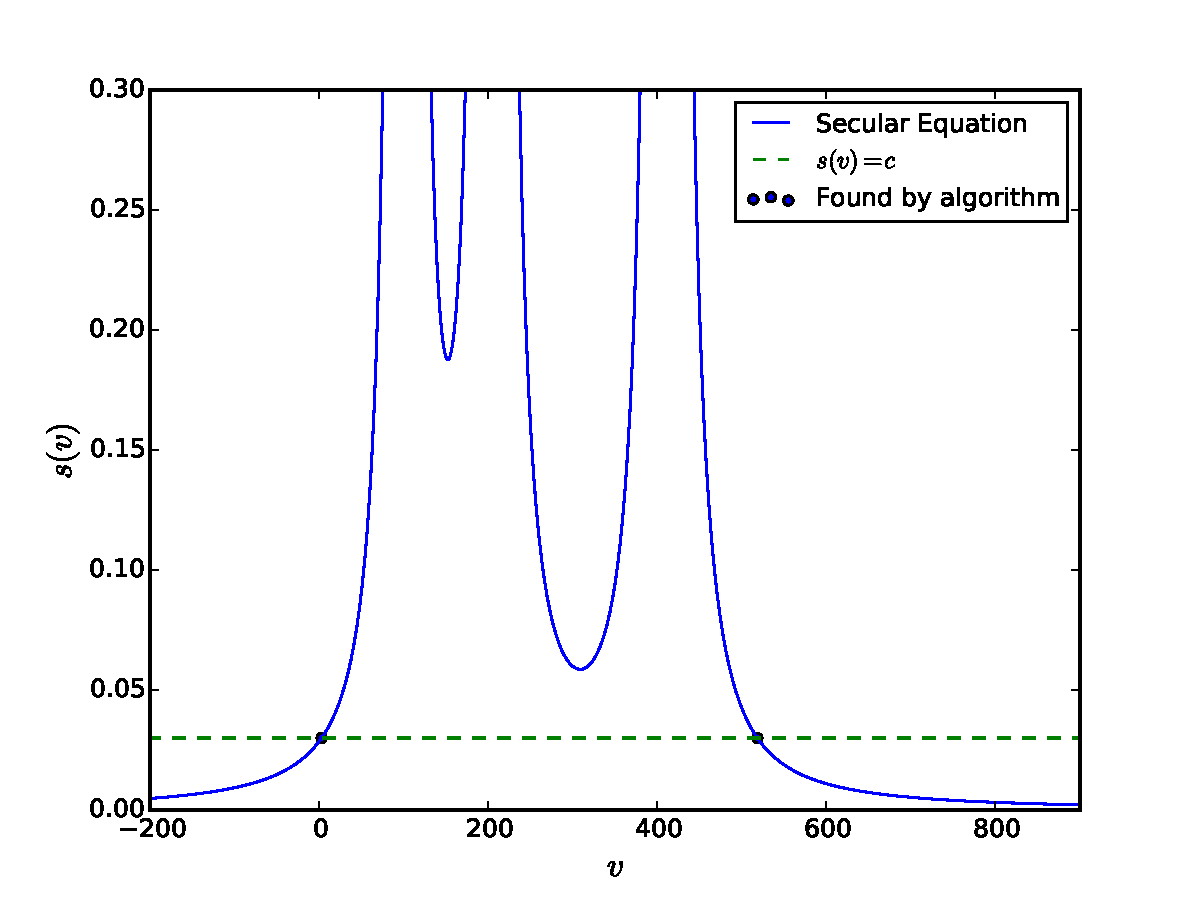
\includegraphics[trim=0.3in 0.in 0.7in 0.4in,clip,width=1\linewidth]{images/secular}
\caption{Secular equation for a single line (corresponding to the instanton) in the RTS-96. Because there were six time steps in the analysis, $s(v)$ approaches infinity at six poles. Dots show the six solutions to $s(v) = c$ identified by our secular equation solver. Note that there could be as few as two solutions if $c$ were small enough.}
\label{fig:secular}
\end{figure}

% TODO: study relationship between secular equation parameters and decision variable values in the original space.

\section{Results}\label{sec:results}
We performed numerical experimentation with three goals in mind. The first is to illustrate the relationship between the instanton pattern and a line's temperature trajectory. How does line temperature evolve in response to instanton angle differences? Second, numerical experimentation can illustrate the effects of wind covariance. What impact does a reasonable covariance matrix have on instanton objective values and wind patterns? The third goal is to characterize algorithm scaling. What is the relationship between the number of wind farms (decision variables) and algorithm performance? How does the solution time of a single QCQP vary with network size and topology?

In every numerical experiment we assumed Waxwing conductors, considered six time steps, and gradually increased the wind forecast over time while keeping conventional generation and demand constant.

\subsection{Temperature Trajectories}
The modified RTS-96 network from \cite{pandzic} provides a helpful test case for illustrating instanton analysis. The network has eighteen wind farms distributed across three areas: nine in the first area, six in the second, and three in the third. Transmission lines are assumed to be Waxwing conductors, as in \cite{almassalkhi2015}. We assume all lines begin at 60 C and have temperature limits of 65 C. We performed instanton analysis for a one-hour time horizon divided into six ten-minute intervals. Figure \ref{fig:temptrajectory} illustrates temperature trajectories corresponding to the instanton and nearby wind patterns. The instanton pattern causes the line to reach 65 C, but if we randomly perturb the instanton pattern while keeping the objective value constant, the line does not reach its temperature limit.

\begin{figure}
\centering
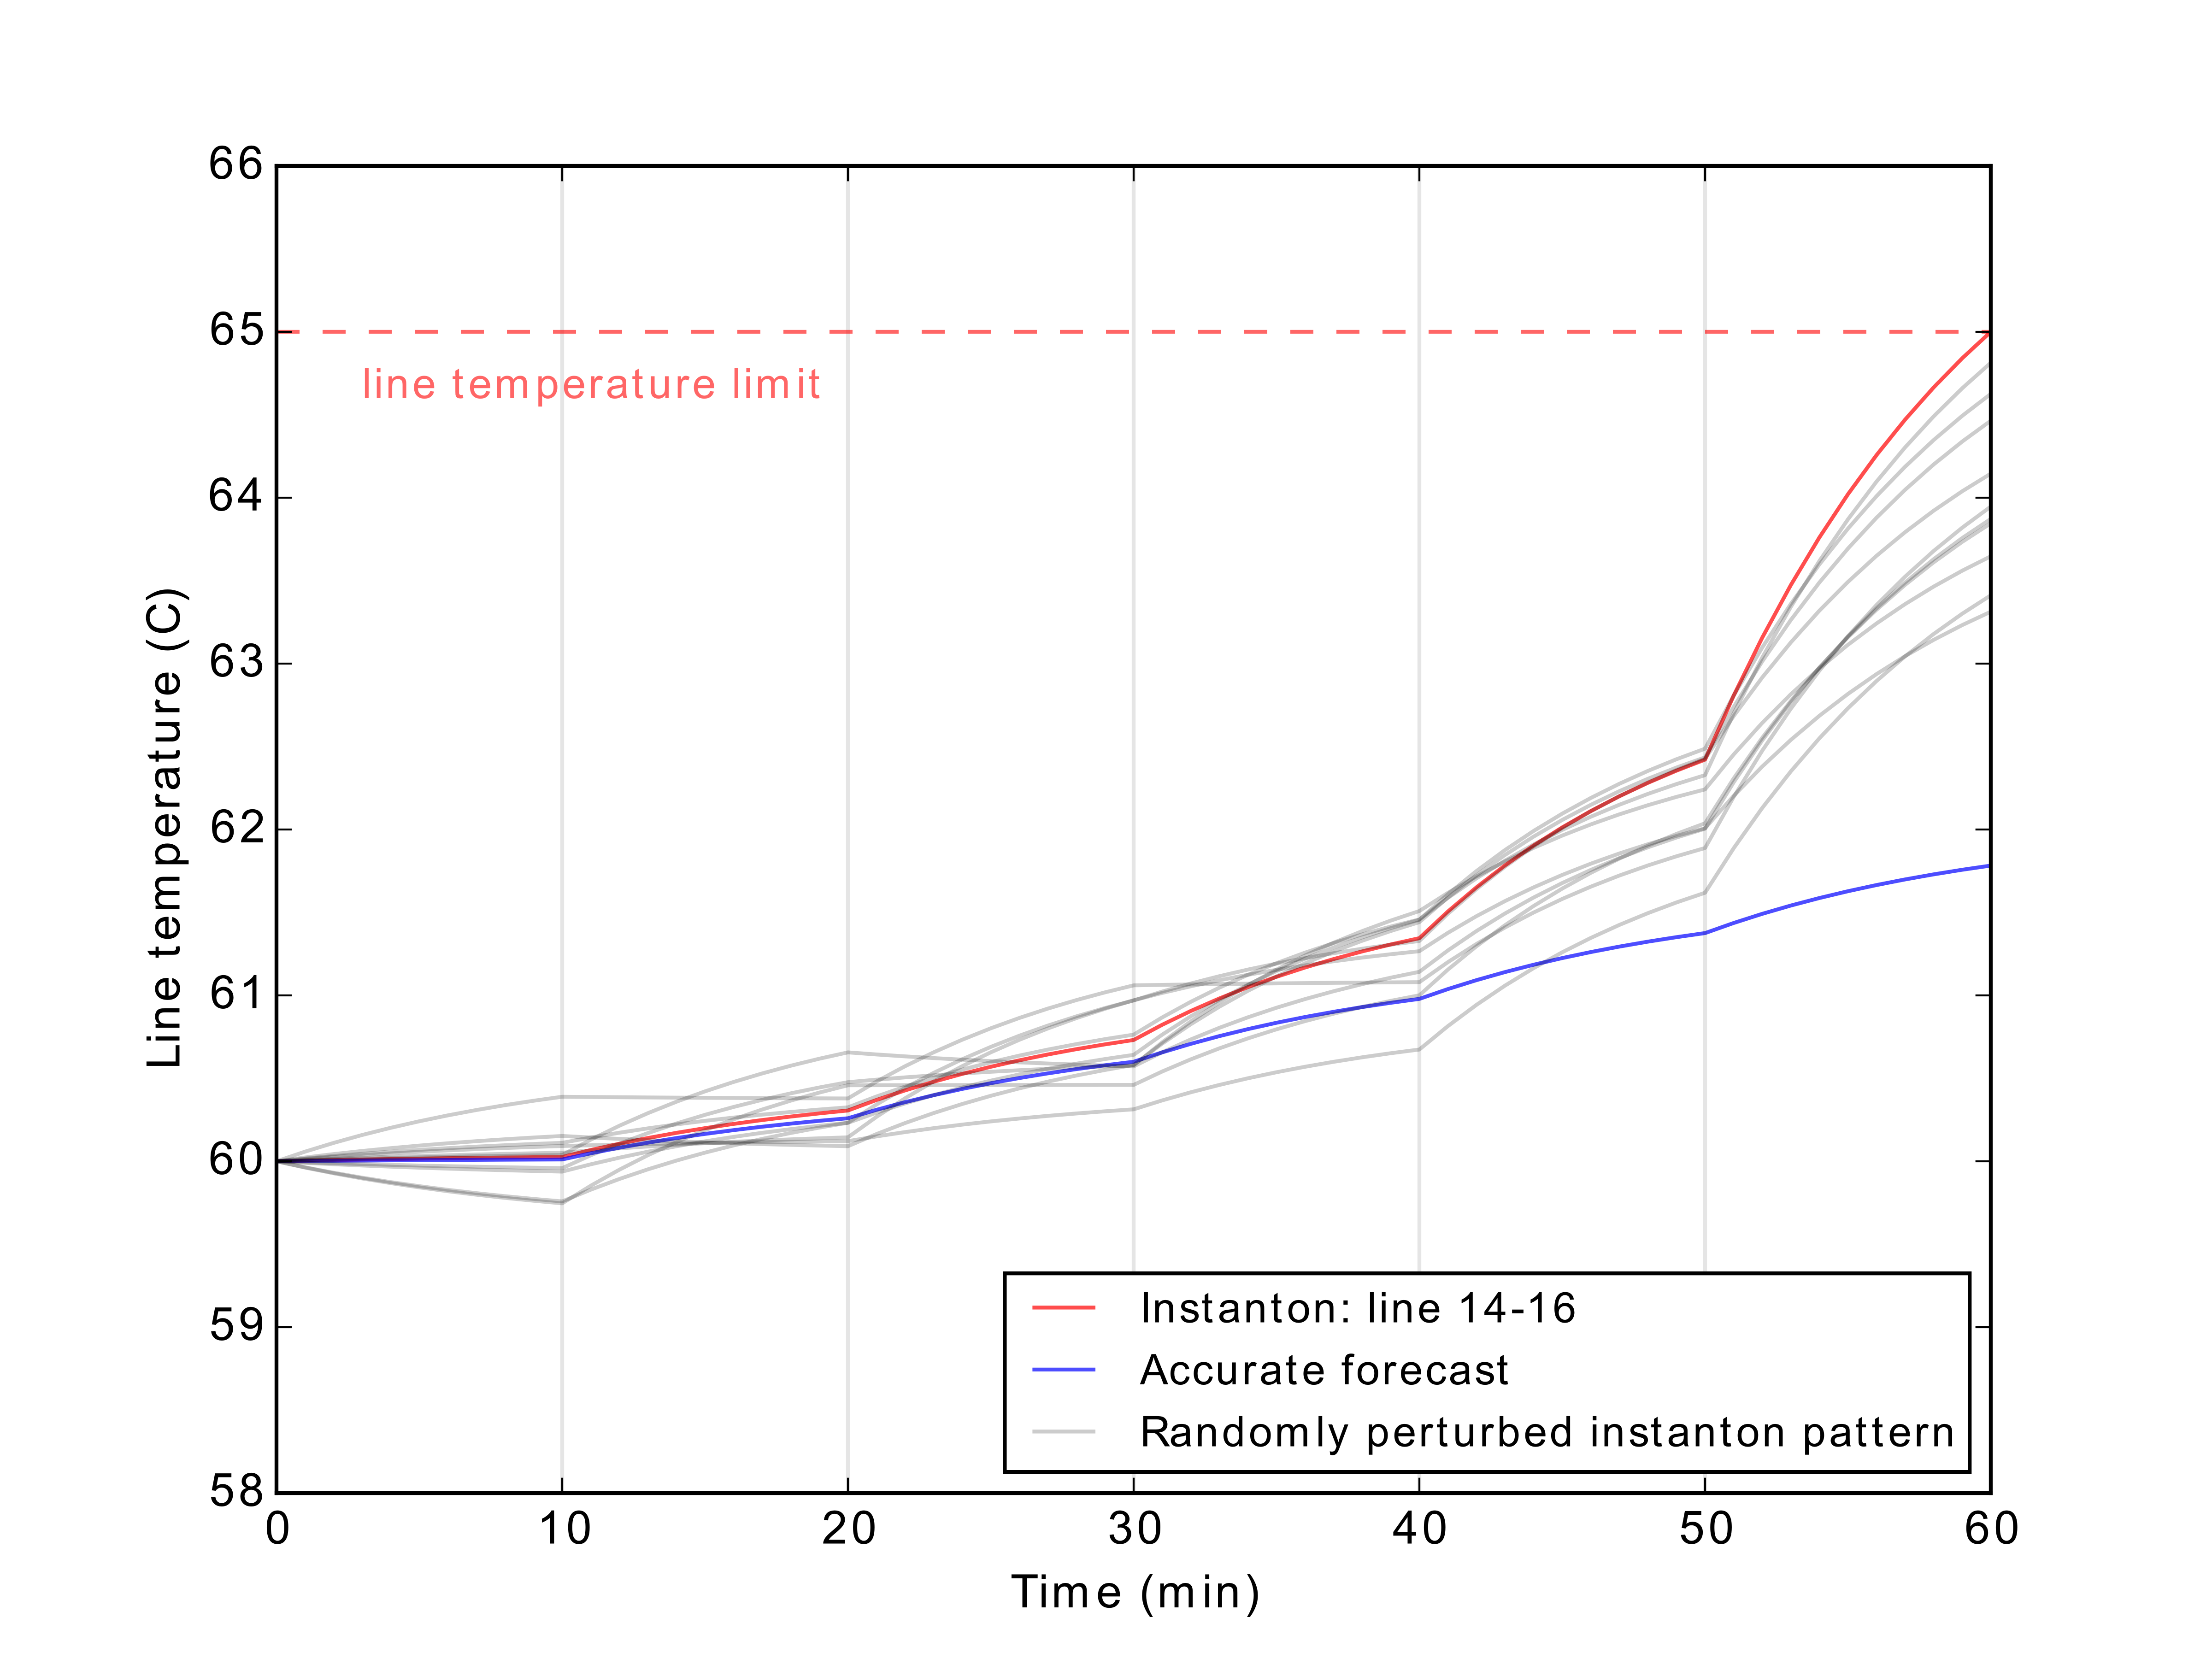
\includegraphics[trim=0.3in 0.in 0.7in 0.4in,clip,width=1\linewidth]{images/temptrajectory}
\caption{RTS-96 temperature trajectories for the line between nodes 14 and 16. Red represents the instanton trajectory, which brings the line to its temperature limit of 65 C. Trajectories shown in gray arise from randomly perturbed versions of the instanton wind pattern having the same objective value. The blue trajectory corresponds to zero deviation from the wind forecast.}
\label{fig:temptrajectory}
\end{figure}

\subsection{Effects of Covariance}
To illustrate the effects of covariance on temporal instanton analysis, we used a simple heuristic method to generate a reasonable spatial covariance matrix for the RTS-96.\footnote{After assigning geographic coordinates to each of the eighteen wind farms and constructing a distance matrix, we mapped distances to correlation coefficients using a relationship from \cite{freris2008}.}

Introducing a positive-definite, unit-norm covariance matrix allows the QCQP solution algorithm to find patterns with lower objective value. Figure \ref{fig:covariance} shows that these patterns have higher objective value when the original objective function (simple two-norm) is used.

\begin{figure}
\centering
\includegraphics[trim=0.3in 0.in 0.7in 0.4in,clip,width=1\linewidth]{images/covariance}
\caption{Objective values for lowest forty instanton candidates, with and without covariance. ``Covariance output measured by norm objective'' was computed by passing solution vectors from the covariance analysis output to the objective function from the no-covariance case.}
\label{fig:covariance}
\end{figure}

\subsection{Algorithm Scaling}
We performed two tests to characterize scaling of our algorithm. First, we varied the number of wind nodes in the RTS-96 network and, considering a time horizon of one hour divided into six equal time intervals, performed a complete analysis in each case. Figure \ref{fig:rts-96-scaling} illustrates the relationship between QCQP size and the time required to perform a complete analysis. Second, we added wind farms to ten of the test cases packaged with MATPOWER \cite{zimmerman2011} and analyzed each. For each network we chose to add a number of wind nodes equal to the number of conventional generators, placed the wind sites randomly, and sized each site to fix wind penetration at $50\%$. The choice of these parameters is somewhat arbitrary for the purposes of characterizing algorithm scaling, but we were careful to add enough significantly-sized wind farms to each network to avoid numerical difficulties.\footnote{If there are too few wind nodes or penetration is too low, many solutions will have absurdly high objective value, and our routine will time out.} Figure \ref{fig:normalized-performance} shows average computation time for a single QCQP versus network size. As a reference point for overall solution time, it took just over two hours for our four-core laptop with 8 GB of RAM to analyze every line in the Polish summer 2008 peak network (case \texttt{3120sp} in Matpower).

\begin{figure}
\centering
\includegraphics[width=1\linewidth]{../images/2015-09-17-rts-96-scaling}
\caption{Total computation time for 119 lines (QCQPs) as a function of total decision variables. The network is the RTS-96, and the time horizon is one hour divided into six ten-minute intervals. Starting with two, the number of wind farms was increased two at a time up to 72 (the network has 73 nodes), and these wind farms were randomly placed throughout the network.}
\label{fig:rts-96-scaling}
\end{figure}

\begin{figure}
\centering
\includegraphics[trim=0in 0in 0in 0in,clip,width=\linewidth]{../images/2015-09-17-normalized-performance-square}
\caption{Average computation time (total time divided by number of lines analyzed) for ten Matpower cases, on a log-log scale. For each network, the number of wind farms is equal to the number of conventional generators, and wind nodes were chosen randomly. In every case the time horizon is five minutes divided into six thirty-second intervals.}
\label{fig:normalized-performance}
\end{figure}

%If the wind farms are concentrated in one portion of the grid, some lines may have instanton candidates with low objective value while other lines have no solutions at all. This may be interpreted in terms of injection shift factors: if shift factors corresponding to the effect of wind injections on a particular line are small, it would take absurd wind forecast deviations to raise that line's temperature from, say, 60 C to 65 C.

\section{Conclusion}\label{sec:conclusion}
This paper has extended the temporal instanton analysis method presented in \cite{kersulis2015} with a focus on implementation and algorithm scaling. A DC-approximate line loss expression allowed us to write a recursive relationship between a line's final and initial temperatures in terms of voltage angle differences during a sequence of discrete time steps.



% needed in second column of first page if using \IEEEpubid
%\IEEEpubidadjcol

% An example of a floating figure using the graphicx package.
% Note that \label must occur AFTER (or within) \caption.
% For figures, \caption should occur after the \includegraphics.
% Note that IEEEtran v1.7 and later has special internal code that
% is designed to preserve the operation of \label within \caption
% even when the captionsoff option is in effect. However, because
% of issues like this, it may be the safest practice to put all your
% \label just after \caption rather than within \caption{}.
%
% Reminder: the "draftcls" or "draftclsnofoot", not "draft", class
% option should be used if it is desired that the figures are to be
% displayed while in draft mode.
%
%\begin{figure}[!t]
%\centering
%\includegraphics[width=2.5in]{myfigure}
% where an .eps filename suffix will be assumed under latex, 
% and a .pdf suffix will be assumed for pdflatex; or what has been declared
% via \DeclareGraphicsExtensions.
%\caption{Simulation results for the network.}
%\label{fig_sim}
%\end{figure}

% Note that IEEE typically puts floats only at the top, even when this
% results in a large percentage of a column being occupied by floats.


% An example of a double column floating figure using two subfigures.
% (The subfig.sty package must be loaded for this to work.)
% The subfigure \label commands are set within each subfloat command,
% and the \label for the overall figure must come after \caption.
% \hfil is used as a separator to get equal spacing.
% Watch out that the combined width of all the subfigures on a 
% line do not exceed the text width or a line break will occur.
%
%\begin{figure*}[!t]
%\centering
%\subfloat[Case I]{\includegraphics[width=2.5in]{box}%
%\label{fig_first_case}}
%\hfil
%\subfloat[Case II]{\includegraphics[width=2.5in]{box}%
%\label{fig_second_case}}
%\caption{Simulation results for the network.}
%\label{fig_sim}
%\end{figure*}
%
% Note that often IEEE papers with subfigures do not employ subfigure
% captions (using the optional argument to \subfloat[]), but instead will
% reference/describe all of them (a), (b), etc., within the main caption.
% Be aware that for subfig.sty to generate the (a), (b), etc., subfigure
% labels, the optional argument to \subfloat must be present. If a
% subcaption is not desired, just leave its contents blank,
% e.g., \subfloat[].


% An example of a floating table. Note that, for IEEE style tables, the
% \caption command should come BEFORE the table and, given that table
% captions serve much like titles, are usually capitalized except for words
% such as a, an, and, as, at, but, by, for, in, nor, of, on, or, the, to
% and up, which are usually not capitalized unless they are the first or
% last word of the caption. Table text will default to \footnotesize as
% IEEE normally uses this smaller font for tables.
% The \label must come after \caption as always.
%
%\begin{table}[!t]
%% increase table row spacing, adjust to taste
%\renewcommand{\arraystretch}{1.3}
% if using array.sty, it might be a good idea to tweak the value of
% \extrarowheight as needed to properly center the text within the cells
%\caption{An Example of a Table}
%\label{table_example}
%\centering
%% Some packages, such as MDW tools, offer better commands for making tables
%% than the plain LaTeX2e tabular which is used here.
%\begin{tabular}{|c||c|}
%\hline
%One & Two\\
%\hline
%Three & Four\\
%\hline
%\end{tabular}
%\end{table}


% Note that the IEEE does not put floats in the very first column
% - or typically anywhere on the first page for that matter. Also,
% in-text middle ("here") positioning is typically not used, but it
% is allowed and encouraged for Computer Society conferences (but
% not Computer Society journals). Most IEEE journals/conferences use
% top floats exclusively. 
% Note that, LaTeX2e, unlike IEEE journals/conferences, places
% footnotes above bottom floats. This can be corrected via the
% \fnbelowfloat command of the stfloats package.


% if have a single appendix:
\appendix[Line Temperature Model]
% or
%\appendix  % for no appendix heading
% do not use \section anymore after \appendix, only \section*
% is possibly needed

\subsection{Heat Balance Equation}
The change in temperature of any object may be expressed as a differential equation called the heat balance equation, which relates temperature change to a sum of various sources of heating. The IEEE 738 standard \cite{ieee2013} provides the following heat balance equation for a transmission line:

\begin{align}\label{eq:heatbalance}
\frac{dT}{dt} &= \frac{1}{m\cdot C_p}\left[I^2\cdot R(T_\text{l,C}(t)) - q_c - q_r + q_s \right]
\end{align}
In \eqref{eq:heatbalance}, $T_\text{l,C}(t)$ is the conductor average temperature in Celsius, $m\cdot C_p$ is the product of mass and heat capacity, and $I^2\cdot R(T_\text{l,C}(t))$ represents heat rate due to resistive heating. $q_c$ represents convective heat loss, which is proportional to the temperature difference between the line and surrounding air:
\begin{align}\label{eq:qc}
q_c &= \eta_c\cdot(T_\text{l,C}(t) - T_\text{a,C})~,
\end{align}
where $T_\text{a,C}$ is the ambient temperature in Celsius. $q_r$ in \eqref{eq:heatbalance} represents radiation heat loss, modeled by the fourth-order expression
\begin{align}\label{eq:qr}
 q_r &= \eta_r\cdot\left[T_\text{l,K}(t)^4 - T_\text{a,K}^4\right],
\end{align}
where $T_\text{l,K}(t)$ and $T_\text{a,K}$ are the conductor and ambient temperatures in Kelvin, respectively. Finally, $q_s$ in \eqref{eq:heatbalance} represents solar heating. In this paper $q_s$ is fixed to some conservative constant (corresponding to full, direct sun).

\subsection{DC Line Loss Approximation}
We replace the resistive heat rate term $I^2\cdot R(T_\text{l,C}(t))$ by $f_{ij}^\text{loss}$, the approximate line loss expression derived in \cite{almassalkhi2014}:
\begin{equation}\label{eq:lossapprox}
f_{ij}^{\text{loss}} \approx r_{ij}\left(\frac{\theta_{ij}}{x_{ij}}\right)^2,
\end{equation}
where $\theta_{ij}$ is the difference between angles $\theta_i$ and $\theta_k$, and $r_{ij} +j x_{ij}$ is the impedance of the line between nodes $i$ and $j$. Three DC power flow assumptions underpin \eqref{eq:lossapprox}: voltage magnitudes are all 1pu, cosine may be approximated by its second-order Taylor expansion, and $x_{ij} \geq 4r_{ij}$. Thus, \eqref{eq:lossapprox} provides an approximate relation between voltage angle difference and line losses.

\subsection{Linearization of Radiation Heat Rate}
When \eqref{eq:heatbalance} is combined with an initial temperature $T_\text{l,C}^0$ and \eqref{eq:lossapprox}, the resulting initial value problem should make it possible to determine conductor temperature $T_\text{l,C}(t_n)$ at a later time $t_n$. We substitute \eqref{eq:qc}-\eqref{eq:lossapprox} into \eqref{eq:heatbalance} and attempt to solve for temperature:
\begin{multline}\label{eq:heatbalance_approx}
\frac{dT}{dt} = \frac{1}{mC_p}\big[ f_{ij}^\text{loss} - \eta_c\left( T_\text{l,C}(t) - T_\text{a,C}\right) \\ - \eta_r\left(T_\text{l,K}(t)^4 - T_\text{a,K}^4\right) + q_s \big]
\end{multline}
If we suppose that power flow, ambient temperature, and solar heat rate are constant, this differential equation is still fourth-order in conductor temperature $T_\text{C}(t)$ due to radiation. Fortunately, $q_r$ is approximately linear over our temperature range of interest (from ambient temperature to temperature limit). We replace $q_r$ by $\tilde{q}_r$, a conservative linearization:\footnote{Because a transmission line is hotter than surrounding air, radiation tends to decrease line temperature. Thus, a conservative approach will underestimate $q_r$. Plotting \eqref{eq:approx_rad} shows that it does indeed underestimate $q_r$.}
\begin{align}\label{eq:approx_rad}
\tilde{q}_r &= \eta_r  \left( T_\text{m,K}^4 - T_\text{a,K}^4\right) +  4\eta_rT_\text{m,K}^3(T_\text{l,C}(t) - T_\text{m,C}),
\end{align}
where $T_\text{m,C}$ is the average (midpoint between) ambient and conductor limit temperatures in Celsius, and $T_\text{m,K}$ is $T_\text{m,C}$ converted to Kelvin. After substitution of \eqref{eq:approx_rad}, the heat balance equation becomes linear in conductor temperature, and the IVP has a straightforward solution.

\subsection{Line Temperature as Recursive Relationship}
Substitution of \eqref{eq:approx_rad} into \eqref{eq:heatbalance_approx} yields the approximate heat balance equation
\begin{align}\label{eq:diffeq}
\frac{dT_\text{l,C}}{dt} &= aT_\text{l,C}(t) + b~,
\end{align}
where constants $a$ and $b$ are defined as
\begin{subequations}
\begin{align}
a &= \frac{1}{mC_p} \left[ -\eta_c - 4\eta_rT_\text{m,K}^3 \right]
\end{align}
\begin{multline}
b = \frac{1}{mC_p} \big[ f_{ij}^\text{loss} + \eta_cT_\text{a,C} - \eta_r \left( T_\text{m,K}^4 - T_\text{a,K}^4 \right) \\ + 4\eta_rT_\text{m,C}\cdot T_\text{m,K}^3 + q_s \big]
\end{multline}
\end{subequations}

The IVP \eqref{eq:diffeq} has a straightforward solution:
\begin{align}\label{eq:tivp}
T_\text{l,C}(t) &= ke^{at} - \frac{b}{a},
\end{align}
where $k=T_\text{l,C}(0) + b/a$. Note that $b$ is influenced by power flow (via
$f_{ij}^\text{loss}$ according to \eqref{eq:lossapprox}), but $a$ is not.

The only variables in \eqref{eq:tivp} are initial temperature and angle differences during each time interval. There is therefore a recursive relationship between final temperature and initial temperature that involves only angle differences. The derivation of this recursive relationship is an exercise in messy linear algebra; it is omitted here for brevity.
%Suppose there are three time intervals: $t_1$, $t_2$, and $t_3$. Then the line temperature at the end of the third interval is given by
%
%\begin{align}
%\nonumber T(t_3) &= k_3 e^{(t_3-t_2)a} - \frac{b_3}{a} \\
%\nonumber &= \left[k_2 e^{(t_2-t_1)a} - \frac{b_2}{a} + \frac{b_3}{a}\right]e^{(t_3-t_2)a} - \frac{b_3}{a} \\
%\nonumber &= \left[\left( T(t_1) + \frac{b_2}{a} \right)e^{(t_2-t_1)a} - \frac{b_2}{a} + \frac{b_3}{a}\right]e^{(t_3-t_2)a} - \frac{b_3}{a} \\
%\label{eq:Texpand} &= \Bigg\lbrace\left[\left(T(t_0) + \frac{b_1}{a}\right) \nonumber e^{(t_1-t_0)a} - \frac{b_1}{a} + \frac{b_2}{a}\right]e^{(t_2-t_1)a} \\
%& \qquad \qquad \qquad \qquad - \frac{b_2}{a} + \frac{b_3}{a}\Bigg\rbrace e^{(t_3-t_2)a} - \frac{b_3}{a}
%\end{align}
%The recursive pattern is apparent. Because all time intervals are the same length, we have
%\begin{align*}
%e^{(t_3-t_2)a} &= e^{(t_2-t_1)a} = e^{(t_1-t_0)a}~,
%\end{align*}
%and we can distribute in \eqref{eq:Texpand} to obtain
%\begin{multline}
%T(t_3) = (e^{(t_1-t_0)a})^3\left(T(t_0) + \frac{b_1}{a}\right) \\ + (e^{(t_1-t_0)a})^2\left(- \frac{b_1}{a} + \frac{b_2}{a}\right) \\ + (e^{(t_1-t_0)a})\left(- \frac{b_2}{a} + \frac{b_3}{a}\right) - \frac{b_3}{a}
%\end{multline}
%Because power flow data enters through $b_1$, $b_2$, and $b_3$, it makes sense to
%group terms accordingly:
%
%\begin{multline}
%T(t_3) = ((e^{(t_1-t_0)a})^3T(t_0) + \\ \left(\frac{(e^{(t_1-t_0)a})^3}{a} - \frac{(e^{(t_1-t_0)a})^2}{a}\right)b_1 \\ + \left( \frac{(e^{(t_1-t_0)a})^2}{a} - \frac{(e^{(t_1-t_0)a})^1}{a}\right)b_2 \\ + \left(\frac{e^{(t_1-t_0)a}}{a} - \frac{1}{a}\right) b_3
%\end{multline}
%The pattern in the above expression makes it easy to extend $T(t_3)$ to cover the general case $T(t_n)$:
%
%\begin{multline}\label{eq:recursive}
%T(t_n) = (e^{(t_1 - t_0)a})^n T(t_0) \\ + \frac{1}{a} \sum_{i=1}^n \left( (e^{(t_1-t_0)a})^i - (e^{(t_1-t_0)a})^{i-1} \right)b_{n-i+1}
%\end{multline}
%
%Ultimately \eqref{eq:recursive} will be used to constrain a line's final temperature to some limiting value. The remainder of this section will relate \eqref{eq:recursive} back to power flow angles so it can be ``plugged in'' to the optimization framework.
%
%\subsection{Relating temperature to angle differences}
%
%Recall that $b_n$ depends on the angle difference at time $t_n$:
%
%\begin{align}
%\nonumber b_n &= \frac{1}{mC_p} \Bigg[ \frac{r_{ij}}{x_{ij}^2}\cdot \frac{S_b}{3L_{ij}} \theta_{ij}(t_n)^2 + \eta_cT_\text{amb} \\
%\nonumber &\qquad - \eta_r\left((T_\text{mid} + 273)^4 - (T_\text{amb} + 273)^4\right) \\
%&\qquad + 4\eta_rT_\text{mid}(T_\text{mid} + 273)^3 + q_s \Bigg] \\
%\label{eq:bexpand} b_n &= c\theta_{ij}(t_n)^2 + d
%\end{align}
%where constants $c$ and $d$ are defined as:
%\begin{align*}
%c &= \frac{r_{ij}S_b}{3 mC_p x_{ij}^2L_{ij}} \\
% d &= \frac{1}{mC_p}\left[ \eta_cT_\text{amb} - \eta_r\left((T_\text{mid} + 273)^4 - (T_\text{amb} + 273)^4\right) + 4\eta_rT_\text{mid}(T_\text{mid} + 273)^3 + q_s \right]
%\end{align*}
%Substitute \eqref{eq:bexpand} into \eqref{eq:recursive}:
%\begin{align*}
%T(t_n) &= (e^{(t_1 - t_0)a})^n T(t_0) + \frac{1}{a} \sum_{i=1}^n \left( (e^{(t_1-t_0)a})^i - (e^{(t_1-t_0)a})^{i-1} \right)(c\theta_{ij}(t_{n-i+1})^2 + d)
%\end{align*}
%Expand the sum term:
%\begin{multline}\label{eq:sumexpand}
%\frac{1}{a} \sum_{i=1}^n \left( (e^{(t_1-t_0)a})^i - (e^{(t_1-t_0)a})^{i-1} \right)(c\theta_{ij}(t_{n-i+1})^2 + d) = \frac{c}{a}\left[ \sum_{i=1}^n \left( (e^{(t_1-t_0)a})^i - (e^{(t_1-t_0)a})^{i-1} \right)\theta_{ij}(t_{n-i+1})^2\right] + \\  \qquad + \frac{d}{a}\left[ \sum_{i=1}^n \left( (e^{(t_1-t_0)a})^i - (e^{(t_1-t_0)a})^{i-1} \right)\right]
%\end{multline}
%Substitute \eqref{eq:sumexpand} into the line temperature equation, introducing the constant $f$ to keep things a bit neater:
%\begin{align}\label{eq:almostthere}
%T(t_n) &= f + \frac{c}{a}\left[ \sum_{i=1}^n \left( (e^{(t_1-t_0)a})^i - (e^{(t_1-t_0)a})^{i-1} \right)\theta_{ij}(t_{n-i+1})^2\right]
%\end{align}
%where
%\begin{align}
%f &= (e^{(t_1 - t_0)a})^n T(t_0) + \frac{d}{a}\left[ \sum_{i=1}^n \left( (e^{(t_1-t_0)a})^i - (e^{(t_1-t_0)a})^{i-1} \right)\right]
%\end{align}
%Rearrange \eqref{eq:almostthere} to isolate angle differences:
%\begin{align}
%\sum_{i=1}^n \left( (e^{(t_1-t_0)a})^i - (e^{(t_1-t_0)a})^{i-1} \right)\theta_{ij}(t_{n-i+1})^2 &= \frac{a}{c}(T(t_n) - f)
%\end{align}
%Now define
%\begin{equation}\label{eq:thetahat}
%\hat{\theta}_{ij}(t_{k})=  \theta_{ij}(t_k)\sqrt{ (e^{(t_1-t_0)a})^{n-k+1} - (e^{(t_1-t_0)a})^{n-k} }
%\end{equation}
%to obtain
%\begin{align}\label{eq:finaltemp}
%\sum_{k=1}^n \hat{\theta}_{ij}(t_{k})^2 &= \frac{a}{c}\left(T(t_n) - f\right)
%\end{align}
%The expression \eqref{eq:finaltemp} may be used to constrain line temperature to be equal to some limiting value by the end of the last time interval.
%
%This derivation has been somewhat messy. The line temperature constraint is summarized in the next section for convenience.




%Comparison with the temperature calculation method recommended by IEEE in \cite{ieee2013} shows th To validate the approximate line temperature model derived here, I compared it to the IEEE 738 standard model using RTS-96 and Waxwing conductor parameters.
%
%\subsection{Summary of IEEE 738 temperature calculation}\label{summary-of-ieee-738-temperature-calculation}
%
%IEEE recommends numerically integrating \eqref{eq:heatbalance} to compute temperature changes. The temporal instanton framework uses approximate DC losses in place of $I^2R(T_\text{avg})$, so we will be integrating the following heat balance equation:
%
%\begin{align}\label{eq:738heatbalance}
%\frac{dT_\text{avg}}{dt} &= \frac{1}{mC_p}\left( r_{ij}\frac{\theta_{ij}^2}{x_{ij}^2}\frac{S_b}{3L_{ij}} - q_c - q_r + q_s\right)
%\end{align}
%
%Heat rates $q_c$ and $q_r$ are calculated according to \eqref{eq:qc} and \eqref{eq:qr}, respectively (copied here for convenience):
%\begin{align*}
%q_c &= \eta_c\cdot(T - T_\text{amb}) \\
%q_r &= \eta_r\cdot((T + 273)^4 - (T_\text{amb} + 273)^4)
%\end{align*}
%All other parameters are constant during temperature calculation. The important thing to keep in mind about IEEE 738 temperature calculation is that it requires numerical integration; there is no analytic temperature solution for \eqref{eq:738heatbalance}. This means one must select an integration time step $\Delta t$. For each step, one computes the change in temperature by multiplying $\Delta t$ by the value of \eqref{eq:738heatbalance} computed at that step. IEEE recommends a step size smaller than 10\% of the conductor thermal time constant\footnote{A typical transmission line thermal time constant is ten minutes, which means IEEE recommends an integration step size of one minute}. A smaller integration step size yields more accurate results.
%
%\subsection{Comparison}\label{comparison}
%
%I used RTS-96 network data and Waxwing conductor parameters to compare IEEE 738 standard temperature calculation to the model derived in Section \ref{transmission-line-heating}. Figure \ref{fig:temp_model_comparison2} shows line temperatures calculated across three ten-minute time intervals, where each interval has a different angle difference (power flow). The angle differences are
%\begin{center}
%\begin{tabular}{c|c}
%	Interval & Angle difference (rad) \\ \hline
%	   1     &          0.09          \\
%	   2     &          0.04          \\
%	   3     &          0.15          \\
%\end{tabular}
%\end{center}
%
%\begin{figure}[h]
%\centering
%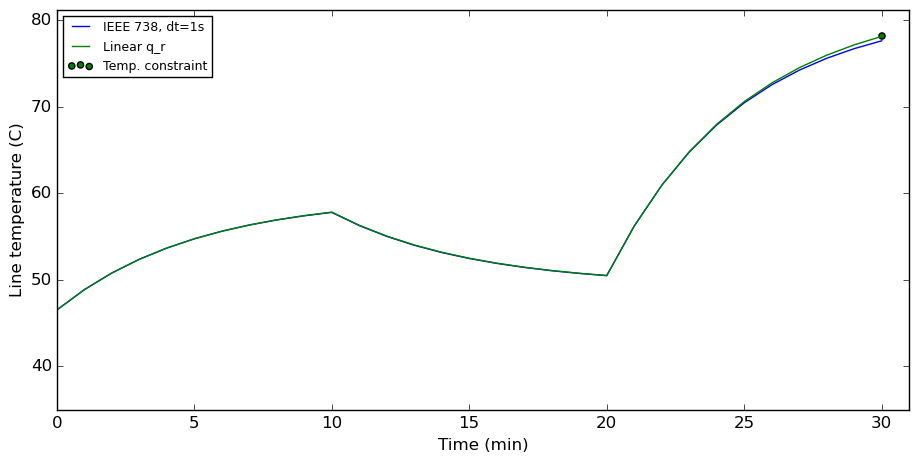
\includegraphics[width=1\linewidth]{../images/temp_model_comparison2}
%\caption{Comparison of IEEE 738 and approximate temperature calculation methods}
%\label{fig:temp_model_comparison2}
%\end{figure}
%
%The blue trace in Figure \ref{fig:temp_model_comparison2} results from numerical integration of \eqref{eq:738heatbalance} with a 1s step size. The green trace comes from the approximate model derived in Section \ref{transmission-line-heating}. The green dot is the final temperature computed by \eqref{eq:almostthere}.
%
%Notes:
%
%\begin{itemize}
%\item
%  Because the approximate line temperature model is analytic (Equation \eqref{eq:tivp} is continuous) while the 738 model requires numerical integration, I chose
%  a very small integration step size of one second to facilitate comparison.
%\item
%  Because the approximate model underestimates the radiative heat loss
%  rate (see Figure \ref{fig:rad_approx}), the green trace should lie slightly above the blue one. This
%  makes the approximate model conservative, which is desirable in the
%  temporal instanton setting. Figure \ref{fig:temp_model_comparison2} illustrates this conservative behavior: the green trace lies on or above the blue trace throughout the time horizon.
%  \item The green dot, computed by \eqref{eq:almostthere}, lies on top of the green curve. This validates the temperature constraint formulation \eqref{eq:tempconstraint}.
%\end{itemize}


%Section \ref{sec:line-losses} describes an approximate line loss formulation that forms the basis of a dynamical model developed in Section \ref{sec:temp-dynamics}. Finally, Section \ref{sec:instanton-formulation} incorporates line temperature dynamics into a complete mathematical model.

%The equations governing AC power flow are nonlinear. If we use these equations to balance the power flows in our optimization, the resulting feasible region will be nonconvex. Previous instanton work has addressed this issue by replacing the AC power flow equations with DC equations (the DC power flow equations assume that the network is lossless, with all voltage magnitudes equal to 1 per unit). This substitution renders the feasible region of instanton optimization (in the absence of nonlinear constraints) convex.

%There are two primary difficulties associated with time-coupled instanton analysis. First, every active and reactive power flow is related to all variables involved in the flow:  the voltage magnitudes at both nodes and the angle difference between them. If we allow this tight coupling into our optimization framework, there will be no guarantee of a unique solution, or indeed of any solution at all. The second difficulty arises from the equation for power loss. Power loss on a line is proportional to the square of the current through it. This nonlinear relationship leads to nonconvexity in the optimization problem's feasible region. In this paper we address the first concern by using the DC power flow, and we sidestep the second difficulty by using a piecewise-continuous convex relaxation of the power loss equation.


%\newcommand{\splitcell}[2][c]{%
%\begin{tabular}[#1]{@{}c@{}}#2\end{tabular}}
%\begin{table}
%\begin{center}
%\caption{Line heating parameters}
%\label{tab:heatparams}
%\begin{tabular}{|c|c|c|}
%	\hline
%	         Parameter           &   Units    &               Description                \\ \hline
%	           $T_s$             &    $s$     &               Sample time                \\ \hline
%	           $mC_p$            & $J/(m\cdot C)$ & \splitcell{Per-unit-length heat capacity\\of the conductor}         \\ \hline
%	          $\eta_c$           & $W/(m\cdot C)$ &     \splitcell{Conductive heat loss \\ rate coefficient}         \\ \hline
%	          $\eta_r$           & $W/(m\cdot C)$ &      \splitcell{Radiative heat loss\\rate coefficient}         \\ \hline
%	       $T^\text{lim}$        &    $C$     &      \splitcell{Line temperature at\\steady-state current limit.}   \\ \hline
%	       $\Delta q_{s,ij}$ & $W/m$ & \splitcell{Solar heat input\\ into conductor} \\ \hline
%	       $\Delta T_\text{amb}$ & C & \splitcell{Change in \\ambient temperature} \\ \hline
%\end{tabular}
%\end{center}
%\end{table}

% The paper will close with a discussion of how other
%components, such as voltage regulators, may affect the formulation.

% use section* for acknowledgment
\section*{Acknowledgment}

The authors would like to thank Dr. M. Chertkov and Dr. S. Backhaus of Los Alamos National Laboratory for discussions and notes that assisted in the transition from instantaneous to temporal settings, and Dr. D. Bienstock for his expertise and practical assistance in the solution of trust region subproblems.

% Can use something like this to put references on a page
% by themselves when using endfloat and the captionsoff option.
%\ifCLASSOPTIONcaptionsoff
%  \newpage
%\fi



% trigger a \newpage just before the given reference
% number - used to balance the columns on the last page
% adjust value as needed - may need to be readjusted if
% the document is modified later
%\IEEEtriggeratref{8}
% The "triggered" command can be changed if desired:
%\IEEEtriggercmd{\enlargethispage{-5in}}

% references section

% can use a bibliography generated by BibTeX as a .bbl file
% BibTeX documentation can be easily obtained at:
% http://www.ctan.org/tex-archive/biblio/bibtex/contrib/doc/
% The IEEEtran BibTeX style support page is at:
% http://www.michaelshell.org/tex/ieeetran/bibtex/
\bibliographystyle{IEEEtran}
% argument is your BibTeX string definitions and bibliography database(s)
\bibliography{bib}
%
% <OR> manually copy in the resultant .bbl file
% set second argument of \begin to the number of references
% (used to reserve space for the reference number labels box)
%\begin{thebibliography}{1}
%
%\bibitem{IEEEhowto:kopka}
%H.~Kopka and P.~W. Daly, \emph{A Guide to \LaTeX}, 3rd~ed.\hskip 1em plus
%  0.5em minus 0.4em\relax Harlow, England: Addison-Wesley, 1999.
%
%\end{thebibliography}

\newpage
% biography section
% 
% If you have an EPS/PDF photo (graphicx package needed) extra braces are
% needed around the contents of the optional argument to biography to prevent
% the LaTeX parser from getting confused when it sees the complicated
% \includegraphics command within an optional argument. (You could create
% your own custom macro containing the \includegraphics command to make things
% simpler here.)
%\begin{IEEEbiography}[{\includegraphics[width=1in,height=1.25in,clip,keepaspectratio]{mshell}}]{Michael Shell}
% or if you just want to reserve a space for a photo:

\begin{IEEEbiography}{Jonas Kersulis}
(S'12) received the B.S. degree in electrical engineering from the University of Missouri-St. Louis, St. Louis, MO USA; and the M.S. degree in Electrical Engineering:Systems from the University of Michigan, Ann Arbor, MI, USA, where he is currently working on his PhD.

His research interests include power system modeling and optimization.

Jonas is a member of the IEEE Power and Energy Society.
\end{IEEEbiography}

\begin{IEEEbiography}{Ian A. Hiskens}
(S'77--M'80--SM'96--F'06) received the B.Eng. degree in electrical engineering and the B.App.Sc. degree in mathematics from the Capricornia Institute of Advanced Education, Rockhampton, Australia, in 1980 and 1983 respectively, and the Ph.D. degree in electrical engineering from the University of Newcastle, Australia, in 1991.

He is the Vennema Professor of Engineering
in the Department of Electrical Engineering and Computer Science, University of Michigan, Ann Arbor, MI, USA. He has held prior appointments in the Queensland electricity supply industry, and various universities in Australia and the United States. His research interests lie at the intersection of power system analysis and systems theory, with recent activity focused largely on integration of renewable generation and controllable loads.

Dr. Hiskens is actively involved in various IEEE societies, and is VP-Finance of the IEEE Systems Council. He is a Fellow of Engineers Australia, and a Chartered Professional Engineer in Australia.
\end{IEEEbiography}

% if you will not have a photo at all:
%\begin{IEEEbiographynophoto}{John Doe}
%Biography text here.
%\end{IEEEbiographynophoto}

% insert where needed to balance the two columns on the last page with
% biographies
%\newpage

%\begin{IEEEbiographynophoto}{Jane Doe}
%Biography text here.
%\end{IEEEbiographynophoto}

% You can push biographies down or up by placing
% a \vfill before or after them. The appropriate
% use of \vfill depends on what kind of text is
% on the last page and whether or not the columns
% are being equalized.

%\vfill

% Can be used to pull up biographies so that the bottom of the last one
% is flush with the other column.
\enlargethispage{-5in}



% that's all folks
\end{document}


